% Template for a Computer Science Tripos Part II project dissertation
\documentclass[12pt,a4paper,twoside, openright, hidelinks]{report}
\usepackage[pdfborder={0 0 0}]{hyperref}
\urlstyle{same}
\usepackage[UKenglish]{babel}
% \usepackage{bibunits}

\usepackage[margin=25mm]{geometry}
\usepackage[skip=2pt]{caption}
\usepackage{verbatim}
\usepackage{docmute} % only needed to allow inclusion of proposal.tex

\usepackage{bookmark}
\usepackage{parskip}
\usepackage{enumitem}
\usepackage{tabularx}
\usepackage{longtable}
\usepackage{multirow}

\usepackage{pdfsync}

\usepackage{xcolor}
\usepackage[multiple]{footmisc}

\usepackage{minted}
\usepackage[justification=centering]{caption}
\newenvironment{code}{\captionsetup{type=listing}}{}

\usepackage{amsmath,amsthm, bm}
\usepackage{mathtools}
\usepackage{blkarray}
\usepackage{amsfonts} 
\usepackage{graphicx} % allows inclusion of PDF, PNG and JPG images
\usepackage{epstopdf}
% \usepackage{auto-pst-pdf} 

\usepackage{rotating}

\graphicspath{{./figs/}}

\raggedbottom                           % try to avoid widows and orphans
\sloppy
\clubpenalty1000%
\widowpenalty1000%

\renewcommand{\baselinestretch}{1.1}    % adjust line spacing to make
                                        % more readable
% \renewcommand{\labelenumii}{\theenumii}
% \renewcommand{\theenumii}{\theenumi.\arabic{enumii}.}
\usepackage{chngcntr}


\usepackage[backend=bibtex, style=numeric,sorting=none]{biblatex}
\addbibresource{references.bib}

%TC:group table 0 1
%TC:group tabular 1 1
%TC:group longtable 1 1

\begin{document}
\counterwithin{listing}{chapter}

%TC:ignore
%%%%%%%%%%%%%%%%%%%%%%%%%%%%%%%%%%%%%%%%%%%%%%%%%%%%%%%%%%%%%%%%%%%%%%%%
\pagestyle{empty}
\thispagestyle{empty}
\pagenumbering{roman}

\rightline{\large{Kamilė Stankevičiūtė}}

\vspace*{60mm}
\begin{center}
\Large
\textbf{Graph neural networks for age prediction from neuroimaging data} \\[5mm]
\large
Computer Science Tripos -- Part II \\[5mm]
Gonville \& Caius College \\[5mm]
2020
\end{center}

%%%%%%%%%%%%%%%%%%%%%%%%%%%%%%%%%%%%%%%%%%%%%%%%%%%%%%%%%%%%%%%%%%%%%%%%%%%%%%
% Proforma, table of contents and list of figures

\pagestyle{plain}
\newpage
\chapter*{Declaration of originality}

I, Kamilė Stankevičiūtė of Gonville \& Caius College, being a candidate for Part II of the Computer Science Tripos, hereby declare that this dissertation and the work described in it are my own work, unaided except as may be specified below, and that the dissertation does not contain material that has already been used to any substantial extent for a comparable purpose.

\bigskip
\leftline{Signed \textit{Kamilė Stankevičiūtė}}

\medskip
\leftline{Date \today}

\chapter*{Proforma}

\begin{tabular}{ll}
Candidate number:   & ?                  \\
Project title:      & Graph neural networks for age prediction from neuroimaging data \\
Examination:        & Computer Science Tripos -- Part II 2020 \\
Word count:         & 10227\footnotemark[1] \\
Lines of code:      & TODO  \\
Project originator: & Mr Tiago Azevedo                        \\
Supervisors:        & Mr Tiago Azevedo, Mr Alexander Campbell \\ 
\end{tabular}
\footnotetext[1]{Counted using the \LaTeX\ Utilities extension in Visual Studio Code.}
\stepcounter{footnote}

% It is quite in order for the Proforma to point out how ambitious the original aims were and how the work completed represents the triumphant consequence of considerable effort against a background of unpredictable disasters. The substantiation of these claims will follow in the rest of the dissertation.

\section*{Original aims of the project}
% At most 100 words describing the original aims of the project.

To implement the population graph paradigm in modelling multi-modal structural  and functional brain imaging data along with non-imaging information of individual patients. Implement and apply different graph neural network architectures – Graph Convolutional Network (GCN) and Graph Attention Network (GAT) – for a subject brain age prediction task. Evaluate the robustness of graph neural networks to noisy and missing data, comparing their performance against each other and with other known benchmarks.

\section*{Work completed}
% At most 100 words summarising the work completed.

\section*{Special difficulties}

None.

\tableofcontents

\newpage
\section*{Acknowledgements}

%%%%%%%%%%%%%%%%%%%%%%%%%%%%%%%%%%%%%%%%%%%%%%%%%%%%%%%%%%%%%%%%%%%%%%%
%TC:endignore

\pagestyle{headings}
\chapter{Introduction}
\pagenumbering{arabic}

% The Introduction should explain the principal motivation for the project. Show how the work fits into the broad area of surrounding Computer Science and give a brief survey of previous related work. It should generally be unnecessary to quote at length from technical papers or textbooks. If a simple bibliographic reference is insufficient, consign any lengthy quotation to an appendix.

% ~500 words

Many of the common neurological and neurodegenerative disorders, such as Alzheimer’s disease, schizophrenia and multiple sclerosis, have been associated with the abnormal patterns of apparent ageing of the brain~\cite{kaufmann2019}. This link has inspired numerous studies in estimation of the apparent brain age using brain imaging data~\cite{franke2019ten}. The resulting \textit{brain age gap} biomarker, defined as the discrepancy between the brain age estimate and the actual chronological age, can be used to understand the biological pathways behind the ageing process, assess an individual’s risk for various brain disorders and identify new personalised treatment strategies.

Current state-of-the-art machine learning approaches for brain age estimation use structural magnetic resonance imaging (MRI) and genetic data, considering each individual brain in isolation, modelling healthy controls separately from individuals with brain disorders, or developing separate models for each sex~\cite{kaufmann2019,niu2019improved}. At the same time, due to high computational complexity and lack of available datasets, few studies consider patterns that are shared across the sub-groups of patients, other important brain imaging modalities such as functional MRI time-series data (cf. Section~\ref{fmri}), and clinical expertise of neurologists and psychiatrists.

This dissertation proposes a customisable end-to-end framework of graph neural network architectures – including graph convolutional~\cite{kipf2017semi} and graph attention~\cite{velickovic2018graph} networks – as one way to combine the richness of structural, functional MRI and non-imaging modalities when predicting the brain age. The neural networks are trained in a semi-supervised manner on a \textit{population graph} representation of patients, where the nodes of the population graph represent subject-specific neuroimaging data, and edges capture pairwise non-imaging similarities between the different subjects. This follows closely the approach presented in the work of Parisot et al.~\cite{parisot2017spectral,parisot2018disease}, where population graphs are used to classify patients as healthy or suffering from Alzheimer's disease or autism spectrum disorder.

Unlike in other state-of-the-art models, graph neural networks trained on population graphs have the potential to learn from the entire cohort of healthy and affected patients of both sexes at once, capturing a wide range of confounding effects and detecting the variation in brain age trends of different sub-populations of subjects.


% \section{Related work}
% \subsection{Population graphs}
% Semisupervised population graphs in Parisot et al. for classifying healthy patients and patients having Mild Cognitive Impairment/Alzheimer's or autism spectrum disorder. These achieve state-of-the-art accuracies around 70\% even for a binary classification task which indicates that brain conditions are generally a complex task. Due to the different nature of the task and different evaluation metrics, this performance cannot be directly compared to the predictive power of the brain age regression task.

% \subsection{Graph neural networks}

% \subsection{Brain age prediction from neuroimaging data}
% Most of current machine learning-based methods for brain age gap prediction work on per-brain basis and do not consider pairwise similarities between patients, not taking into account the population as a whole.

% Graphs are static so it makes sense that most practical approaches would not use this as their model, because it prevents using applying it for new patients

% Kaufmann et al.~\cite{kaufmann2019} uses gradient boosting based techniques (XGBoost)~\cite{chen2016xgboost} for brain age gap prediction from structural magnetic resonance imaging (MRI) data. The study uses a significantly larger dataset of 45,000 people and presents separate models for female and male brain age gap prediction, without considering any pairwise similarities between individuals.

% Another framework for brain age gap prediction is based on Gaussian Processes regression, using raw T1-weighted MRI scans, segmenting them and using principal components analysis (PCA) for dimensionality reduction~\cite{cole2018brain}.


\chapter{Preparation}
% Principally, this chapter should describe the work which was undertaken before code was written, hardware built or theories worked on. It should show how the project proposal was further refined and clarified, so that the Implementation stage could go smoothly rather than by trial and error.
% Throughout this chapter and indeed the whole dissertation, it is essential to demonstrate that a proper professional approach was employed.
% The nature of this chapter will vary greatly from one dissertation to another but, underlining the professional approach, this chapter will very likely include a section headed “Requirements Analysis” and incorporate other references to software engineering techniques.
% The chapter will cite any new programming languages and systems which had to be learnt and will mention complicated theories or algorithms which required understanding.
% It is essential to declare the Starting Point (see Section 7). This states any existing codebase or materials that your project builds on. The text here can commonly be identical to the text in your proposal, but it may enlarge on it or report variations. For instance, the true starting point may have turned out to be different from that declared in the proposal and such discrepancies must be explained.

%  ~2,500 words


This chapter presents in more depth the brain age estimation problem (Section~\ref{brain-age-estimation}) and the dataset used for the brain age estimation task (Section~\ref{dataset}). It also gives background on population graphs (Section~\ref{population-graphs}) as well as the neural network architectures for implementing them (Sections~\ref{training-gcn} and~\ref{training-gat}).

\section{Brain age estimation}
\label{brain-age-estimation}

The \textit{brain age} is defined as the \textit{apparent} age of the brain tissue, compared to the person's true (or \textit{chronological}) age. For example, a highly atrophied brain of a young person may appear to have a higher brain age than a healthy brain of an older person, because gradual atrophy is related to the normal brain ageing process. 

Following the formal framework of Niu et al.~\cite{niu2019improved}, the brain age $y_b$ can be expressed as the sum of the known chronological age $y_c$ and the unknown \textit{brain age gap} $\varepsilon_g$ that is defined as the discrepancy between the chronological and the brain age:

\begin{equation}
    \label{brainage:eq1}
    y_b = y_c + \varepsilon_g.
\end{equation}

It is generally assumed~\cite{franke2019ten} that a typical healthy person has a normally ageing brain, so the brain age corresponds to chronological age:

\begin{equation}
    \label{brainage:assume}
    y_b \approx y_c.
\end{equation}

Our goal is to estimate brain age $y_b$ as a function $f$ of brain imaging features $X$:

\begin{equation}
    \label{brainage:eq2}
    y_b = f(X) + \varepsilon_e,
\end{equation}

where $\varepsilon_e$ is the prediction error, while the estimate of \textit{chronological} age is instead (from Equations~\eqref{brainage:eq1} and~\eqref{brainage:eq2})

\begin{align}
    y_c &= f(X) + \varepsilon,
        \label{brainage:eq3}
\end{align}

where $\varepsilon \coloneqq \varepsilon_e - \varepsilon_g$ is the error term consisting of both the brain age gap and the model prediction error.

Since the true brain age is unknown, any (semi-)supervised machine learning model can only use chronological age as predicted variable, following Equation~\eqref{brainage:eq3}. However, if the model is trained on healthy subjects only, $f(\cdot)$ can explain both the apparent brain age \textit{and} the true chronological age with $X$, since for healthy subjects $y_b \approx y_c$ (Equation~\eqref{brainage:assume}) and any variance in $\varepsilon$ is assumed to contain just the prediction error. When the same model is applied to non-healthy patients, $f(\cdot)$ explains the chronological age assuming the brain is healthy, and any \textit{additional} unexplained variance in $\varepsilon$ is assumed to be the brain age gap. On the other hand, if the model is trained  on both healthy and non-healthy subjects to predict chronological age, it might learn the confounding effects of both normal (chronological) ageing, and disease-related (brain) ageing, thus hiding the brain age gaps~\cite{dukart2011age}.

An alternative method, which does not restrict training data only to healthy subjects, is proposed in Niu et al.~\cite{niu2019improved}. However, it requires experimentally verifying (e.g. through subjects' performance in cognitive behaviour tests) that $\varepsilon$ depends primarily on the brain age gap $\varepsilon_g$ and not the brain age prediction error $\varepsilon_e$, which is out of the scope of this dissertation.

\section{Dataset}
\label{dataset}

For this project I will use the The United Kingdom Biobank (UKB)~\cite{sudlow2015uk}, which is a continuous population-wide study of over 500,000 participants containing a wide range of measurements. Of particular relevance to this dissertation are the UKB participants with structural and functional magnetic resonance imaging (MRI) data, a total of 17,550 subjects. The features that have been extracted from these subjects are explained in more detail in this section. 


\subsection{Structural features}

Structural MRI is used to analyse the anatomy of the brain. Its two main modalities are the two types of an MRI image called T1-weighted and T2-weighted FLAIR, where each type emphasises different aspects of the scan and highlights some features more than the others (see Figures~\ref{figure:t1} and~\ref{figure:t2} for T1 and T2-weighted MRI images respectively). The structural features used in this project – \textit{cortical thickness}, \textit{surface area} and \textit{grey matter volume} (see Table~\ref{table:structural-features}) – have been extracted from structural MRI images using the Human Connectome Project (HCP) Freesurfer pipeline (see Glasser et al.~\cite{glasser2013minimal} for further discussion of features and preprocessing steps). 

\begin{table}[]
\centering
    \caption{Summary of the features derived from structural MRI, reported separately for every brain region.}\label{table:structural-features}
    
    \begin{tabular}{lp{11cm}}
        \hline
    \textbf{Structural feature}            & \textbf{Description} \\ \hline
    Cortical thickness &  Average thickness of the cerebral cortex in a brain region. \\
    Surface area       &  Surface area of the cerebral cortex in a brain region. \\
    Grey matter volume &  Total volume of the grey matter component of a brain region. \\ \hline
    \end{tabular}
\end{table}

\begin{figure}[]
    \centering
    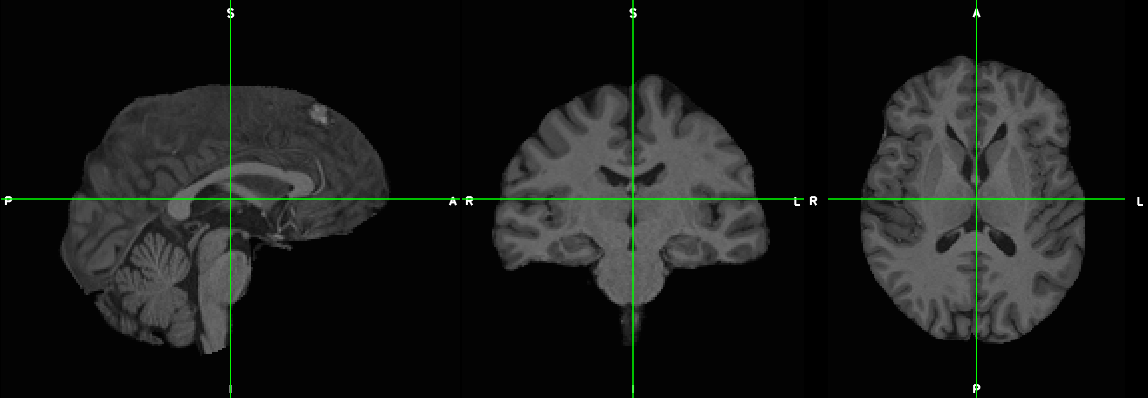
\includegraphics[width=\textwidth]{T1.png}
    \caption{The slices of the T1-weighted MRI image.}\label{figure:t1}
\end{figure}


\begin{figure}[]
    \centering
    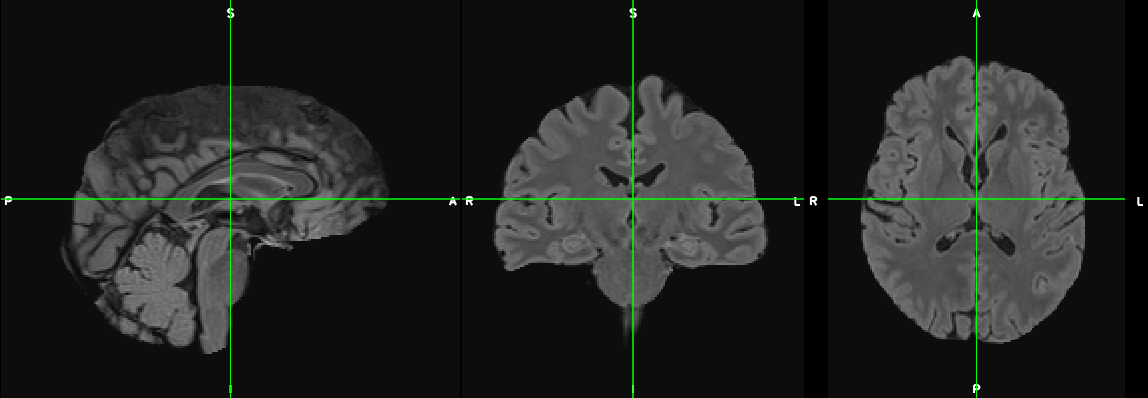
\includegraphics[width=\textwidth]{T2.png}
    \caption{The slices of the T2-weighted FLAIR MRI image.}\label{figure:t2}
\end{figure}


\subsection{Functional features}
\label{fmri}

Functional MRI (fMRI) data indirectly measures brain activity over time. It is represented by \textit{blood oxygenation level dependent} (BOLD) time-series (Figure~\ref{figure:fmri}) that show changes in oxygenation of the blood vessels. Sudden increases in oxygen demand are related to higher brain activity in the corresponding brain region.

The two types of an fMRI image are \textit{task} fMRI, when the subject is asked to perform a specific cognitive task, and \textit{resting state} fMRI (rs-fMRI), when the subject is not performing any particular task. This project will use rs-fMRI data.

For the purposes of machine learning analysis, \textit{functional connectivity matrices} will be derived from rs-fMRI and used as input features to the graph neural network models. Functional connectivity is estimated by correlating the time-series of every pair of brain regions together under the assumption that parts of the brain that have related functions would also have similar activity patterns (highly correlated time-series). 


% As a consequence, we would expect higher correlation between the corresponding BOLD time-series. For time-series $T_1$ and $T_2$, \textit{Pearson's correlation} (denoted as $r$) is computed as

% \begin{equation}
%     r(T_1, T_2) = \frac{\mathrm{cov}(T_1, T_2)}{\sigma_{T_1} \sigma_{T_2}}
% \end{equation}

% where $\mathrm{cov}(\cdot, \cdot)$ denotes covariance and $\sigma$ stands for standard deviation.

% The correlations are used to derive the \textit{functional connectivity matrix} storing pairwise correlations between the different voxels (or parcels) as the overall representation of functional brain connectivity. For time-series $T_1, \dots, T_N$,

% \begin{equation}
%     \mathrm{fcm}(T_1, \dots, T_N) = \begin{bmatrix}
%         r(T_1, T_1) & \cdots & r(T_1, T_N) \\
%         \vdots & \ddots & \vdots \\
%         r(T_N, T_1) & \cdots & r(T_N, T_N)
%     \end{bmatrix},
% \end{equation}

% of which (due to symmetry and the non-informative diagonal) only the flattened lower triangle is usually used as input for the downstream machine learning analysis.


% Could include (Pearson's, lasso, partial correlation, covariance)

% Tiago's observation that partial correlation may give better results when including functional MRI time-series in the machine learning model.
% From wiki on partial correlation: In probability theory and statistics, partial correlation measures the degree of association between two random variables, with the effect of a set of controlling random variables removed. If we are interested in finding whether or to what extent there is a numerical relationship between two variables of interest, using their correlation coefficient will give misleading results if there is another, confounding, variable that is numerically related to both variables of interest. This misleading information can be avoided by controlling for the confounding variable, which is done by computing the partial correlation coefficient. This is precisely the motivation for including other right-side variables in a multiple regression; but while multiple regression gives unbiased results for the effect size, it does not give a numerical value of a measure of the strength of the relationship between the two variables of interest.

\begin{figure}[]
    \centering
    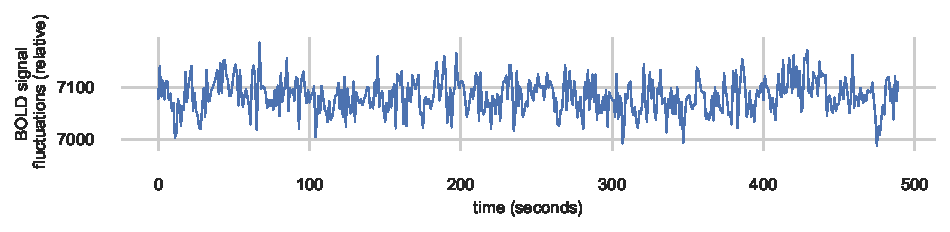
\includegraphics[width=\textwidth]{fmri.pdf}
    \caption{The example BOLD time series.}\label{figure:fmri}
\end{figure}

\subsection{Euler indices}
Euler index\footnote{\url{https://www.ncbi.nlm.nih.gov/pubmed/29278774}} is a quality control metric which represents the number of times the Freesurfer brain reconstruction software failed to seamlessly connect two 2D slices of an MRI image into the 3D representation of the brain. The higher the Euler index, the worse is the quality of the scan. Euler indices might be used to remove the subjects with low-quality scans to avoid them affecting the analysis~\cite{kaufmann2019}. Alternatively, they can be used as a covariate in a machine learning model (as a brain similarity metric or a node feature) to correct for any scan quality-related bias in prediction. This project will use Euler indices as node features for consistency in keeping neuroimaging features in nodes and non-imaging features in edges.


\subsection{Neuroimaging data preprocessing}

All MRI and fMRI data in UKB was preprocessed (denoised and motion-corrected) with standard UK Biobank pipelines\footnote{\url{https://biobank.ctsu.ox.ac.uk/crystal/crystal/docs/brain_mri.pdf}}. For the purpose of this study, the data was further \textit{parcellated} at the Department of Psychiatry by Dr Richard Bethlehem, Dr Rafael Romero-Garcia and Dr Lisa Ronan\footnote{\url{https://github.com/ucam-department-of-psychiatry/UKB}}.

A \textit{parcellation} splits an image of a brain into biologically meaningful regions for downstream analysis, compressing per-voxel\footnote{A \textit{voxel} is a discrete volumetric element.} measurements into per-parcel summaries (see Figure~\ref{figure:parcellated-brain} for an example). In this dissertation, the neuroimaging data will be parcellated with one of the most common parcellations developed by Glasser et al.~\cite{glasser2016multi}, which divides the brain into 360 cortical regions and 16 subcortical regions. 



\begin{figure}[]
    \centering
    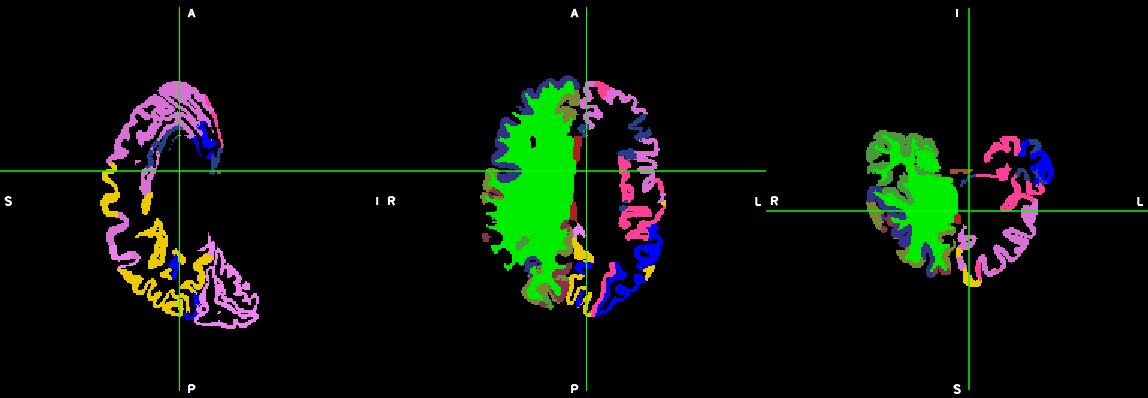
\includegraphics[width=\textwidth]{parcellated_brain.png}
    \caption{The slices of the MRI image with parcels highlighted in different colours.}\label{figure:parcellated-brain}
\end{figure}

% When the brain is imaged there is a choice whether to warp the image of the brain to the fixed atlas or whether to warp the atlas to match the variable brain images. The former makes it easier to process a dataset of many images and find the matching regions of two brains faster, but the latter remains more faithful to the unique structure of the individual patient's brain. 

\subsection{Non-imaging features}

In this dissertation, non-imaging data refers to all subject data that does not come from MRI scans. The features useful to this project include the subject's binary (biological) sex, the psychiatric disorder diagnoses, mental health status, education, and other variables that might have a confounding effect on structure and functional connectivity of the brain~\cite{ruigrok2014meta} and consequently affect the brain age. Table \ref{table:phenotype-features} summarises the non-imaging features selected for this project.

\begin{table}[h]
    \caption{Summary of the non-imaging features used in this project.}\label{table:phenotype-features}
    \centering
    \begin{tabular}{cp{6cm}p{7.5cm}}
        \hline
    \textbf{Code} & \textbf{Non-imaging feature} & \textbf{Explanation} \\ \hline
    \texttt{AGE} & Chronological age &  Used as the training label. \\
    \texttt{FI} & Fluid intelligence score &  Measures cognitive performance. Related to increased brain activity~\cite{gray2003neural}. \\
    \texttt{FTE} & Years of full-time education &  Associated with brain age gaps~\cite{steffener2016differences} and other brain health conditions~\cite{brayne2010education}.\\
    \texttt{ICD10} & Mental and brain health (from ICD10 diagnosis code data) & Subject mental health and nervous system disease diagnoses that might affect the structure and function of the brain. Diagnoses were grouped by categories following the ICD10 system\footnote{\url{https://icd.who.int/browse10/2019/en}}. \\
    \texttt{MEM} & Prospective memory result & Memory generally declines with age, and is related to changing brain activity patterns~\cite{grady2000changes, kliegel2006delayed}. \\
    \texttt{SEX} & Binary sex (male or female) & Highly affects the size and volume of the brain~\cite{ruigrok2014meta}. \\ \hline
    \end{tabular}
\end{table}

The non-imaging data is used to compute the inter-subject similarity score, which will determine the edges of the population graph.

\section{Population graphs}
\label{population-graphs}

One useful way to combine the multiple types of neuroimaging data and represent the relations between subjects for downstream machine learning tasks is a \textit{population graph} data structure, as it is presented by Parisot et al.~\cite{parisot2018disease}.

The set of $N$ subjects $S$ is connected into an undirected population graph $G = (V, E)$, where $V$ is the set of graph nodes (with one node uniquely representing one subject), and $E$ is the set of edges (representing the similarity of subjects).

Each node $v \in V$ is a vector containing the individual subject's neuroimaging data, whether structural, functional, or both. The edge $(v, w) \in E$ connects subjects $s_v, s_w \in S$ based on some \textit{similarity metric} that uses the non-imaging information of the subjects to create edges between the nodes. 

Defining a good similarity metric is important to correct for the confounding effects on the feature vectors (e.g. the subject's sex affects the brain volume) as well as to cluster subjects into the most informative neighbourhoods. For example, in this dissertation the neighbourhoods that have similar brain age gaps could be useful. If carefully defined, the similarity metrics could include the domain expertise of neurologists and psychiatrists as well.

Similarity metrics are defined using a \textit{similarity function} $\mathrm{sim}(\cdot, \cdot)$ which takes two subjects and returns the similarity score between them (the higher the score, the more similar are the subjects):

\begin{equation}
    \mathrm{sim}(s_v, s_w) = \frac{1}{n}\sum_{i=1}^{n} \mathbf{1}[M_i(s_v) = M_i(s_w)].
    \label{eq:similarity}
\end{equation}

Here $\{M_1, \dots, M_n\}$ is a set of non-imaging features that are used to compute subject similarity and $\mathbf{1}[\cdot]$ is an indicator function, in this case returning a non-zero value when the values for a given non-imaging feature $M_i$ match for the two subjects $s_v$ and $s_w$. In practice, if the metric is a real number, ``matching'' could be defined in terms of non-imaging features being within some constant $\epsilon > 0$. 

To avoid memory issues when $|E| \sim O(N^2)$ and minimise the size of the neighbourhood to only highly similar subjects, a \textit{similarity threshold} $\mu$ is used such that

\begin{equation}
    (v, w) \in E \iff \mathrm{sim}(s_v, s_w) \geq \mu.
    \label{eq:similarity-threshold}
\end{equation}

The population graphs can only be effectively accepted as input to machine learning models that are capable of operating on graph-structured data. The two following sections will discuss two types of \textit{graph neural networks} (GNNs) that will be implemented in this dissertation for this purpose, namely graph convolutional and graph attention networks.

\section{Graph convolutional networks}
\label{training-gcn}
% What is actually essential about the graph convolutional networks?

One of the approaches how the graphs can be represented in neural networks is based on spectral graph theory~\cite{hammond2011wavelets}. The main advantage of this strategy is that it makes the operations applied to every node independent of the local graph topology (the number of neighbours of a particular node). This is easier to optimise as the same operation can be applied to all nodes. 

The graph is therefore first transformed from spatial (Euclidean) to spectral (Fourier) domain. The more expensive convolution operation in the Euclidean domain corresponds to a cheaper multiplication operation in the Fourier domain.

\subsection{Graph spectral decomposition}

In spectral analysis, a graph $G = (V, E)$ is represented by its \textit{normalised graph Laplacian} matrix~\cite{defferrard2016convolutional}: 

\begin{equation}
    \mathbf{L} = \mathbf{I} - \mathbf{D}^{-1/2}\mathbf{A}\mathbf{D}^{-1/2},
\end{equation}

where $\mathbf{I}$ is the identity matrix, $\mathbf{D} \in \mathbb{N}^{N \times N}$ is the diagonal degree matrix of the graph nodes, and $\mathbf{A} \in \{0, 1\}^{N \times N}$ is the adjacency matrix such that $a_{ij} = \mathbf{1}[(i, j) \in E]$. The graph Laplacian uniquely represents the graph as it is based on the graph's topology.

The positive semidefinite graph Laplacian matrix is decomposed as

\begin{equation}
    \mathbf{L} = \mathbf{U\Lambda U}^\mathrm{T},
\end{equation}

where $\mathbf{\Lambda}$ is the diagonal eigenvalue matrix, and $\mathbf{U}$ is the eigenbasis defining the graph Fourier domain: for a signal $\mathbf{x} \in \mathbb{R}^{F}$ (e.g. a graph node with $F$ features), $\mathbf{\hat{x}} = \mathbf{U}^\mathrm{T}\mathbf{x}$ is the \textit{graph Fourier transform} of $\mathbf{x}$, and $\mathbf{x} = \mathbf{U}\mathbf{\hat{x}}$ is its inverse~\cite{wu2019simplifying}.

% Eigenvalues as graph frequencies and learning as a low-pass filter of frequencies.
% Fourier transform as transformation to the eigenbasis obtained through graph Laplacian diagonalisation.

%~\cite{velickovic2018graph}: graph definition in the Fourier domain based on the eigendecomposition of the graph Laplacian

\subsection{Spectral graph convolution}

For a filter $\mathbf{g} \in \mathbb{R}^m$ with a diagonal matrix $\mathbf{\hat{G}} = \mathrm{diag}(\mathbf{U}^\mathrm{T}\mathbf{g})$ containing the filter's spectral coefficients, the graph convolution of a signal $\mathbf{x}$ is defined as

\begin{equation}
    \label{eq:convolution}
    \mathbf{x} *_G \mathbf{g} = \mathbf{U}((\mathbf{U}^\mathrm{T}\mathbf{x}) \odot (\mathbf{U}^\mathrm{T}\mathbf{g})) = \mathbf{U}\mathbf{\hat{G}}\mathbf{U}^\mathrm{T}\mathbf{x}
\end{equation}

where $\odot$ is the element-wise (Hadamard) product~\cite{wu2019simplifying}.

\subsection{Optimising graph convolutions}
This section reviews the steps towards optimised graph convolutional networks (GCNs) as proposed by Kipf and Welling~\cite{kipf2017semi}.

\subsubsection{ChebNets}
To avoid the $O(N^2)$ filtering operation due to the matrix-vector multiplications in Equation~\eqref{eq:convolution}, Defferrard et al.'s~\cite{defferrard2016convolutional} ChebNets use recursively defined \textit{Chebyshev polynomials}

\begin{gather}
    T_k(\mathbf{M}) = 2\mathbf{M}T_{k-1}(\mathbf{M}) - T_{k-2}(\mathbf{M}) \\
    T_1 = \mathbf{M} \\
    T_0 = \mathbf{I}
\end{gather}

to approximate the filter $\mathbf{\hat{G}}$ as 

\begin{equation}
    \mathbf{\hat{G}} \approx \sum_{k = 0}^{K} \theta_k T_k(\mathbf{\tilde{\Lambda}})
\end{equation}

where $\mathbf{\tilde{\Lambda}} = 2\mathbf{\Lambda}/\lambda_{\mathrm{max}} - \mathbf{I}$, $\lambda_\mathrm{max}$ is the largest eigenvalue in $\mathbf{\Lambda}$, and $\theta_k$ are coefficients such that $\mathbf{\hat{G}} = \sum_k \theta_k \mathbf{\Lambda}^k$~\cite{wu2019simplifying}. The truncation coefficient (polynomial order) $K$ corresponds to the neighbourhood of at most $K$ hops away from the node of interest, and such convolution is said to be $K$-localised. 

Next, it can be proved~\cite{wu2019comprehensive} that

\begin{equation}
    T_k(\mathbf{\tilde{L}}) = \mathbf{U}T_k(\mathbf{\tilde{\Lambda}})\mathbf{U}^{\mathrm{T}}
\end{equation}

with $\mathbf{\tilde{L}} = 2\mathbf{L}/\lambda_{\mathrm{max}} - \mathbf{I}$. The result is the approximated spectral graph convolution:

\begin{equation}
    \label{eq:chebnet}
    \mathbf{x} *_G \mathbf{g} \approx \sum_{k=0}^{K}\theta_k T_k(\mathbf{\tilde{L}})\mathbf{x}.
\end{equation}

% ChebNet: filters further approximated by Chebyshev expansion of the graph Laplacian avoiding the expensive eigendecomposition operation (ChebNet) (velickovic)

\subsubsection{GCNs}
Kipf and Welling's GCNs~\cite{kipf2017semi} introduce further optimisations to ChebNets: 
\begin{enumerate}
    \item Taking $K=1$ makes Equation~\eqref{eq:chebnet} linear, which is more suitable for neural network architectures with linear layers and non-linearities between them.
    \item To minimise the number of trainable parameters, $\theta_0$ and $\theta_1$ become functions of a single parameter $\theta$: $\theta = \theta_0 = -\theta_1$.
    \item Further assuming $\lambda_{\mathrm{max}}\approx 2$ simplifies the computation of $\mathbf{\tilde{L}}$, since this eliminates the need for eigendecomposition of the Laplacian: $\mathbf{\tilde{L}} = 2\mathbf{L}/\lambda_{\mathrm{max}} - \mathbf{I}$ becomes $\mathbf{\tilde{L}} \approx \mathbf{L} - \mathbf{I}$.
\end{enumerate}

This results in convolution approximation:

\begin{align}
    \mathbf{x} *_G \mathbf{g} &\approx \theta_0 T_0(\mathbf{\tilde{L}}) \mathbf{x} + \theta_1 T_1(\mathbf{\tilde{L}}) \mathbf{x} \\
    &\approx \theta \mathbf{I} \mathbf{x} - \theta (\mathbf{L} - \mathbf{I}) \mathbf{x} \\
    \label{eq:gcnconv1}
    &= \theta(\mathbf{I} + \mathbf{D}^{-1/2}\mathbf{A}\mathbf{D}^{-1/2})\mathbf{x}
\end{align}

Finally, to avoid the numerical instability of repeated convolutions due to the eigenvalues of the matrix in Equation~\eqref{eq:gcnconv1} ranging in $[0, 2]$, a \textit{renormalisation trick} is applied by adding self-loops to the graph nodes: taking $\mathbf{\tilde{A}} = \mathbf{A} + \mathbf{I}$ and $\mathbf{\tilde{D}}$ the degree matrix of $\mathbf{\tilde{A}}$, 

\begin{equation}
    \label{eq:gcnconv2}
    \mathbf{x} *_G \mathbf{g} \approx \theta(\mathbf{\tilde{D}}^{-1/2}\mathbf{\tilde{A}}\mathbf{\tilde{D}}^{-1/2})\mathbf{x}.
\end{equation}
 
% (this citation also very good for follow through for what the training is doing for all layers in general rather than a single feature vector, i.e. the training flow)
% can also mention~\cite{wu2019comprehensive};

% extension: an alternative to Chebyshev polynomials (extension): cayleynet--probably too difficult to implement

\subsection{Graph convolutional layer}
The graph convolution operation in Equation~(\ref{eq:gcnconv2}) is generalised to the entire layer of the network as follows. 

Let $\mathbf{H}^{(l-1)} \in \mathbb{R}^{N\times C_{l-1}}$ be the input layer of a neural network with $C_{l-1}$ input channels, $\mathbf{H}^{(l)} \in \mathbb{R}^{N\times C_{l}}$ be the GCN layer with $C_{l}$ output channels, and $\mathbf{H}^{(0)} = \mathbf{X} \in \mathbb{R}^{N \times C_0}$ containing $C_0$ input features for each of the $N$ nodes in the population graph (in this case the neuroimaging data for $N$ subjects). For the weight matrix $\mathbf{\Theta}^{(l)} \in \mathbb{R}^{C_{l-1}\times C_{l}}$ and an activation function $\sigma(\cdot)$,

\begin{equation}
    \mathbf{H}^{(l)} \leftarrow \sigma( \mathbf{\tilde{D}}^{-1/2}\mathbf{\tilde{A}}\mathbf{\tilde{D}}^{-1/2}\mathbf{H}^{(l-1)}\mathbf{\Theta}^{(l)}).
\end{equation}

\section{Graph attention networks}
\label{training-gat}

In contrast to the \textit{spectral} GCN that relies on the computation within the Fourier domain using the graph Laplacian, the graph attention network (GAT)~\cite{velickovic2018graph} is a \textit{spatial} architecture that operates in the Euclidean domain. Here, the mechanism that incorporates the neighbourhood information is defined to work on the neighbourhoods of different sizes, with each node learning how much importance (\textit{attention}) it should assign to each one of its neighbours.

% \textit{Self-attention} is also added in to the concept where different parts of the node's neighbourhood are considered with different importance weights, getting a representation of the rest of the neighbourhood. 

\subsection{Graph attentional layer}
Analogously to the previous section, we consider an input layer $\mathbf{H}^{(l-1)} \in \mathbb{R}^{|V|\times C_{l-1}}$ (with $\mathbf{H}^{(0)} = \mathbf{X} \in \mathbb{R}^{|V|\times C_{0}}$ as before) and the GAT layer $\mathbf{H}^{(l)} \in \mathbb{R}^{|V|\times C_{l}}$. Denote the input layer $\mathbf{H}^{(l-1)}$ as $[\mathbf{h}_1^{(l-1)} \cdots \mathbf{h}_{|V|}^{(l-1)}]^{\mathrm{T}}$, and $\mathbf{H}^{(l)}$ as $[\mathbf{h}_1^{(l)} \cdots \mathbf{h}_{|V|}^{(l)}]^{\mathrm{T}}$. For a trainable weight matrix $\mathbf{W}^{(l)} \in \mathbb{R}^{C_{l} \times C_{l-1}}$ and an \textit{attentional mechanism} $a: \mathbb{R}^{C_{l}} \times \mathbb{R}^{C_{l}} \rightarrow \mathbb{R}$ we compute (unnormalised) \textit{attentional coefficients} $e_{ij}$:

\begin{equation}
    e_{ij} = a(\mathbf{W}^{(l)}\mathbf{h}_i^{(l-1)}, \mathbf{W}^{(l)}\mathbf{h}_j^{(l-1)}).
\end{equation}

In Veli{\v{c}}kovi\'{c} et al.~\cite{velickovic2018graph}, the attention mechanism is implemented as a linear transformation using a learnable weight vector $\mathbf{a} \in \mathbb{R}^{2C_{l}}$, followed by a non-linearity $\mathrm{LeakyReLU}(\cdot)$ with slope 0.2 for negative input:

\begin{align}
    e_{ij} &= a(\mathbf{W}^{(l)}\mathbf{h}_i^{(l-1)}, \mathbf{W}^{(k)}\mathbf{h}_j^{(l-1)}) \\
    &= \mathrm{LeakyReLU}(\mathbf{a}^{\mathrm{T}}[\mathbf{W}^{(l)}\mathbf{h}_i^{(l-1)} \parallel \mathbf{W}^{(l)}\mathbf{h}_j^{(l-1)}]),
\end{align}

where $\parallel$ denotes concatenation.

The graph topology is accounted for by discarding any coefficients $e_{ij}$ where $(i, j) \notin E$, and normalising the coefficients $\alpha_{ij}, (i, j) \in E$ for the rest using the softmax function:

\begin{align}
    \alpha_{ij} &= \underset{{j: (i, j) \in E}}{\mathrm{softmax}}\left(e_{ij}\right) \\
    &= \underset{{j: (i, j) \in E}}{\mathrm{softmax}}\left(\mathrm{LeakyReLU}(\mathbf{a}^{\mathrm{T}}[\mathbf{W}^{(l)}\mathbf{h}_i^{(l-1)} \parallel \mathbf{W}^{(l)}\mathbf{h}_j^{(l-1)}])\right) \\
    &=  \frac{\mathrm{exp}\left(\mathrm{LeakyReLU}(\mathbf{a}^{\mathrm{T}}[\mathbf{W}\mathbf{h}_i^{(l-1)} \parallel \mathbf{W}^{(l)}\mathbf{h}_j^{(l-1)}])\right)}{\sum\limits_{k: (i, k) \in E}\mathrm{exp}\left(\mathrm{LeakyReLU}(\mathbf{a}^{\mathrm{T}}[\mathbf{W}^{(l)}\mathbf{h}_i^{(l-1)} \parallel \mathbf{W}^{(l)}\mathbf{h}_k^{(l-1)}])\right)}.
\end{align}

The coefficients $\alpha_{ij}$ and the weight matrix are used to compute the output features for another non-linearity $\sigma$:

\begin{equation}
    \label{eq:attention}
    \mathbf{h}_i^{(l)} = \sigma\left(\sum\limits_{j: (i, j) \in E} \alpha_{ij}\mathbf{W}^{(l)}\mathbf{h}_j^{(l-1)}\right)
\end{equation}

\subsection{Multi-head attention}
The above attention mechanism can be repeated several times to stabilise the performance, where one independent application of attention is called an \textit{attention head}. The outputs of the independent attention heads are concatenated or averaged together until the last layer of the complete neural network architecture when they are averaged into a single output. For $M$ attention heads, the results of Equation~\eqref{eq:attention} are concatenated in non-final layers:

\begin{equation}
    \mathbf{h}_i^{(l)} = \underset{m=1}{\overset{M}{\big\|}} \sigma\left(\sum\limits_{j: (i,j)\in E} \alpha_{ij, m}\mathbf{W}^{(l)}_m\mathbf{h}_j^{(l-1)}\right),
\end{equation}

or averaged if GAT is the final ($L$-th) layer of the network:

\begin{equation}
    \mathbf{h}_i^{(L)} = \sigma\left(\frac{1}{M}\sum\limits_{m=1}^M\sum\limits_{j: (i,j)\in E} \alpha_{ij, m}\mathbf{W}^{(L)}_m\mathbf{h}_j^{(L-1)}\right).
\end{equation}

\section{Training task}
\label{training-task}
% Train/validation/test split, cross-validation, patient selection and exclusion from results, stratification, graph representation (edge lists, node features, edge features,...)

% Labels are available for a small subset of nodes and are spread across neighbourhoods through a regularisation term such as Laplacian~\cite{kipf2017semi}, predicting the labels for the remaining nodes

For node label prediction tasks such as brain age estimation, the population graphs are trained in a \textit{semi-supervised} manner: while the entire dataset (every node and edge) is included in the graph, only a subset of the nodes is labelled, with the goal being to learn the labels for the remaining nodes~\cite{kipf2017semi}. At each training step (epoch), the feedback from nodes with available labels is used to update the parameters for the entire graph, which could be seen as information being ``propagated'' from a labelled node to the neighbours that are similar to it (as defined by the similarity metric). After the model is trained, every node in the population graph has a prediction for its label.

The predictive power of a model can be evaluated based on its performance on a set of test nodes, for which the labels had been invisible to the model at the training stage. For the brain age estimation task, the metrics used to evaluate the performance are Pearson's correlation $r$ and coefficient of determination $r^2$~\cite{niu2019improved}.


% TODO \textit{an illustration of the graph with marked training and validation nodes with visible labels and how the training happens on those followed by how the graph is evaluated on the test nodes where the parameters were updated but the labels never seen} – maybe include in GCN/GAT sections instead?

% TODO illustrations could also explain the operation of the networks, perhaps highlighting differences between GCN and GAT graphically: Averaging representations of neighbour features and smoothing labels as a consequence.~\cite{wu2019simplifying}


\section{Requirements analysis}
\label{section:requirements-analysis}

The project has three main stages that directly correspond to the Success Criteria of the Project Proposal (Appendix~\ref{chapter:project-proposal}):

\begin{enumerate}[label=S\arabic*.]
    \item Implementation of the population graph data structure, with nodes containing the individual neuroimaging data and edges representing associations between them based on pairwise similarity. This involves: \begin{enumerate}[label=\theenumi\arabic*.]
        \item Preprocessing of the functional, structural imaging and non-imaging data of the UKB subjects.
        \item Implementation of the customisable similarity metric that would compare two subjects and return the similarity score.
        \item A pipeline that would generate the population graph for a given set of subjects, their modalities, similarity metric and similarity threshold.
        \item An \textit{extension} for supporting higher flexibility in similarity metrics by including the similarity score as an edge feature rather than having a 1-weighted edge whenever the similarity score exceeds a given threshold.
    \end{enumerate}
    \item Implementation of the graph convolutional network (GCN) and graph attention network (GAT) architectures for the age regression task. 
    \item Training and evaluation of the two graph neural network architectures on the UKB population graph. This includes the \textit{extension} of implementing the robustness measurement framework.
\end{enumerate}

I expect stage S1 to be the most complex for the following additional requirements.
\begin{enumerate}[label=R\arabic*.]
    \item Care must be taken to make sure that the data is handled \textit{correctly}. This will require testing of the components which transform the data to the population graph data structure.
    \item The pipeline must be \textit{flexible} enough to support the various combinations of modalities, subjects, and similarity metrics, which will be ensured by independent support of every modality and the \textit{extension} of the project to support custom similarity functions.
    \item The pipeline has to be \textit{modular} enough to be easily extended to more datasets, modalities and processing options in the future. To achieve this, the pipeline will be split into independent components with their own designated function, so that they are easier to build upon independently.
\end{enumerate} 

These considerations by themselves largely fulfil the proposed \textit{extension} of implementing the pipeline that can handle raw data at the one of its earliest processing stages in an end-to-end manner – indeed any earlier stage would require advanced neuroimaging processing expertise that would be out of scope of a Part II project. 

The full design of the neuroimaging processing pipeline with respect to those requirements, as well as the GCN and GAT architectures and their evaluation, is discussed in Chapter~\ref{chapter:implementation}.

\section{Software engineering practice}
Since every stage discussed in the previous section depends on the implementation of the previous one, the straightforward workflow is to carry out the three stages in order (except for the extensions, which would be implemented last). This fits best with the \textit{waterfall model} of software development because the project is relatively small and has a straightforward set of requirements, the design of the pipeline directly corresponds to the three project stages, and implementation depends on how the different pipeline stages are designed to interact with each other. Chapter~\ref{chapter:implementation} walks through the schematic design diagrams that were used as foundation for the component implementation.

To track the workflow, prevent loss of data and ease the readability and/or any future extensions to this project, the common practices of consistent code style (adhering to PEP8\footnote{\url{https://www.python.org/dev/peps/pep-0008/}} style guide), comprehensive documentation, unit testing, code reuse, version control (through a \texttt{git} repository), and backup strategies (regular backups to an external disk, GitHub repository, Google Drive) will be applied.

\section{Choice of tools}

Because of its popularity and wide community support in both machine learning and neuroimaging, I chose Python as the implementation language for this interdisciplinary project.

This project will use \textit{PyTorch Geometric}~\cite{fey2019pytorch}, a popular extension library for \textit{PyTorch}~\cite{pytorch} that provides out-of-the-box graph neural network architecture implementations and has the advantage over other libraries (and other machine learning frameworks such as TensorFlow) of being easy to learn and use. 

The neuroimaging machine learning library \textit{Nilearn} will be used for some of the neuroimaging data processing and visualisation~\cite{abraham2014machine, nilearn}.

For scientific computing, I will use common Python packages such as \textit{scikit-learn}~\cite{pedregosa2011scikit}, \textit{pandas}~\cite{mckinney2010scipy}, and \textit{NumPy}~\cite{walt2011numpy}. 

For testing, I will use Python's \texttt{unittest} library.

For model logging, visualisation and hyperparameter tuning, I will use the free \textit{Weights~\& Biases}~\cite{wandb} framework because of its clean, intuitive interface and automated machine learning capabilities.


\section{Starting point}
The discussion of the architectures proposed in this section assumes the knowledge of the Computer Science Tripos courses relating to scientific computing, artificial intelligence, machine learning, and information theory. The conceptual understanding of the brain age estimation, neuroimaging data processing and graph neural networks (none of which I had previous experience with) required the study of papers cited as well as other supporting resources.

The code builds on implementations provided by the packages listed in the previous section. I had no previous experience with most of them.

The preprocessed dataset has been provided by Dr Richard Bethlehem of Department of Psychiatry.

\chapter{Implementation}
% This chapter should describe what was actually produced: the programs which were written, the hardware which was built or the theory which was developed. Any design strategies that looked ahead to the testing stage might profitably be referred to (the professional approach again).
% Descriptions of programs may include fragments of high-level code but large chunks of code are usually best left to appendices or omitted altogether. Analogous advice applies to circuit diagrams.
% Draw attention to the parts of the work which are not your own. The Implementation Chapter should include a section labelled ”Repository Overview”. The repository overview should be around one page in length and should describe the high-level structure of the source code found in your source code Repository. It should describe whether the code was written from scratch or if it built on an existing project or tutorial. Making effective use of powerful tools and pre-existing code is often laudable, and will count to your credit if properly reported.
% It should not be necessary to give a day-by-day account of the progress of the work but major milestones may sometimes be highlighted with advantage.

%  ~4,500 words

% Tangent works better than correlation or partial correlation.
\section{Overview}

\begin{figure}[]
    \centering
    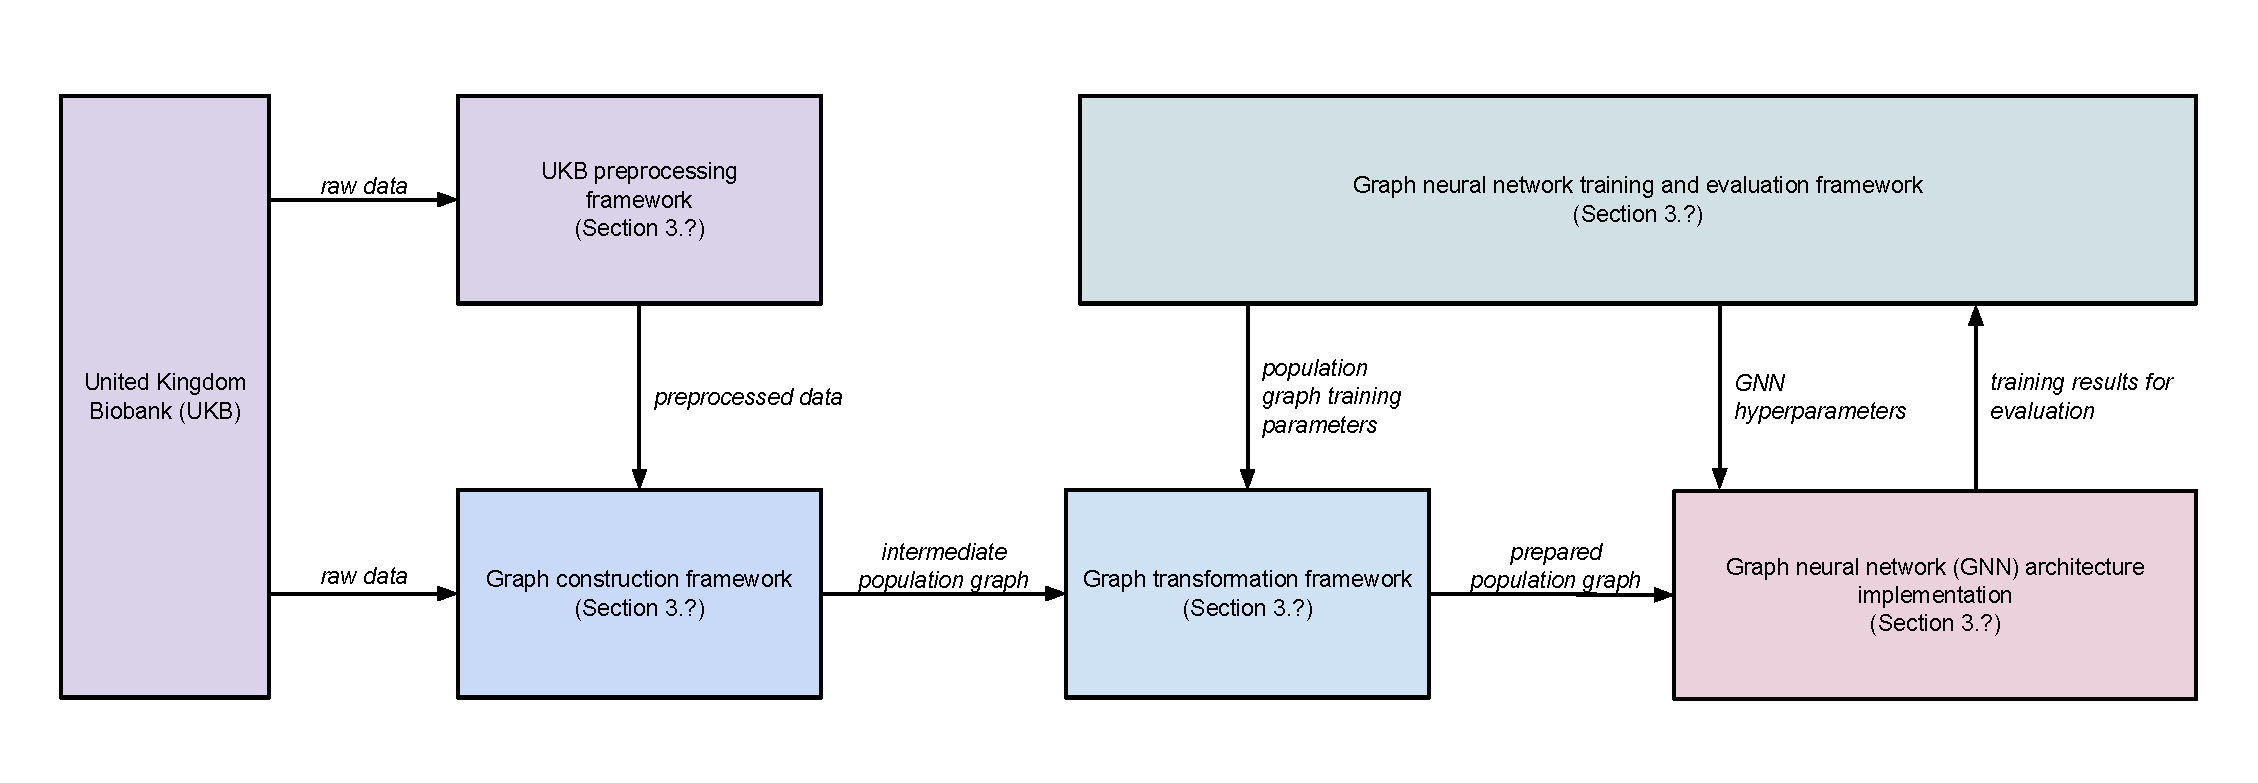
\includegraphics[width=\textwidth]{pipeline_overview.pdf}
    \caption{Overview of the key project components.}\label{pipeline-overview}
\end{figure}

This project can be divided into five key components, as illustrated in Figure~\ref{pipeline-overview}:
\begin{enumerate}
    \item Preparation of the United Kingdom Biobank (UKB) dataset;
    \item Intermediate population graph construction;
    \item Population graph transformation for training;
    \item Training on graph neural network architectures;
    \item Evaluation of the graph neural network performance.
\end{enumerate}

The work was split into these particular components so that each of them can carry out a single task independently of the other parts of the program, (other than the clearly defined input/output communication). This makes the overall project easier to implement, understand and extend in the future, generalising it to other datasets and preprocessing methods. 

This chapter will explain in detail the implementation behind each of the components.

\section{UKB preprocessing component}

The main function of the UKB preprocessing component is to prepare the raw or partially preprocessed UKB data for population graph construction. In particular, to improve the computational efficiency of operations later in the pipeline (potentially saving hours or days of computation time), this component preprocesses the data in a convenient form. This involves filtering the dataset, precomputing similarity matrices and functional connectivity matrices. The schematic diagram of these steps is shown in Figure~\ref{preprocessing-component}, which will be referred to throughout this section.

\begin{figure}[h]
    \centering
    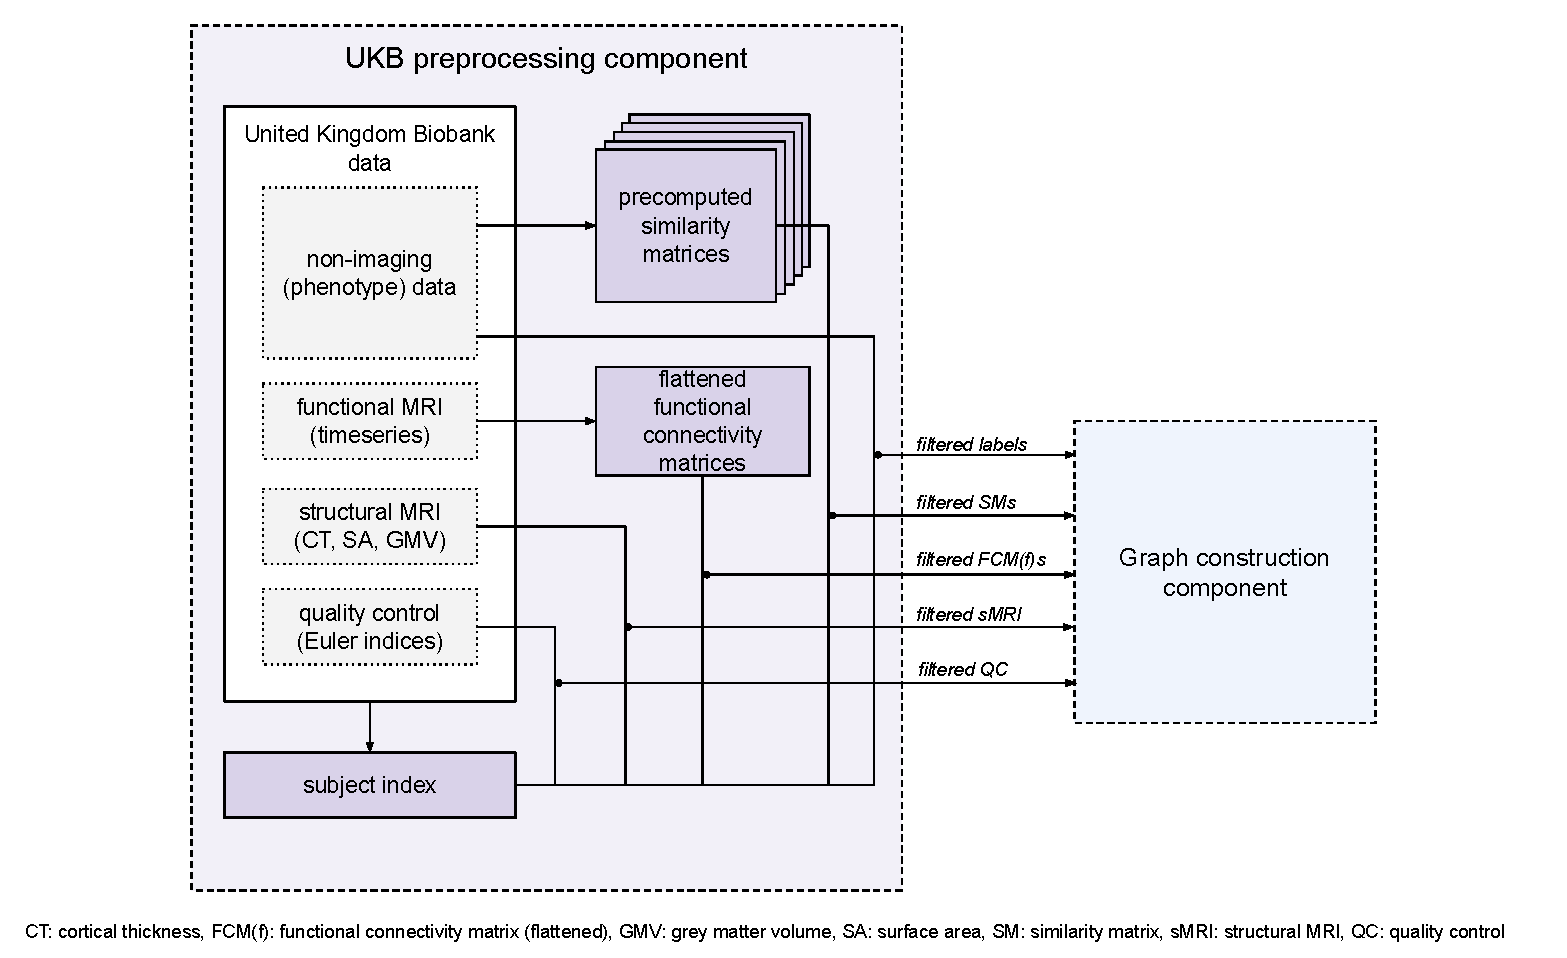
\includegraphics[width=\textwidth]{preprocessing_component.pdf}
    \caption{Overview of the UKB preprocessing component.}\label{preprocessing-component}
\end{figure}

\subsection{Cleaning the dataset}
The different modalities of the UKB data, shown in the white box in Figure~\ref{preprocessing-component}, have been provided separately from each other, with a small minority of subjects having the data available for some of the modalities but not others (for example due to data corruption or its retraction by the participant). To ensure consistent and smooth processing, the subjects with partially missing data (236 in total) have been excluded from further processing. The remaining 17,314 subjects with well-defined modalities have been collected into a \textit{subject index} (purple box on the bottom left), which was used to filter the data before its collection to the population graph construction component.

\subsection{Precomputing connectivity matrices}
The connectivity matrices involve computing pairwise correlations of 376 time-series (for 360 cortical and 16 subcortical regions) for every subject. With 20 gigabytes of raw timeseries data across over 17,000 subjects, this introduces a high computational overhead (a few hours on a CPU) if the matrices are computed on the fly as the graph is constructed. An additional inefficiency comes from the computation being repeated whenever a population graph that uses the functional data is constructed. To avoid this, the matrices are computed once for each subject, flattened and their lower triangles stored as \texttt{numpy} arrays as part of the preprocessing component.

% TODO could include the maths here?

\subsection{Precomputing similarity matrices}
The computation of pairwise similarity scores is quadratic in both time and space with respect to the number of subjects. Depending on the exact method how the similarity function is computed, a general-purpose (non-accelerated) processor might take hours or even days to process the entire dataset. This computation is also repeated whenever a graph is constructed, since the similarities per non-imaging metric do not change over different population graphs: the variation comes from different selections of subjects, non-imaging features, their relative weighting, and similarity thresholds.

The similarity matrices – one for each non-imaging feature in Table~\ref{table:phenotype-features} – have therefore been computed in advance. Unlike the functional connectivity data that is used directly for population graph node features (and therefore should avoid redundancy), the feature-wise similarity matrices are sliced and filtered depending on the selection of subjects. In this case it is more practical to store the full matrix, so that the integer indices into the similarity matrix directly correspond to the subject index in other components of the population graph data structure (see Section~\ref{section:population-graph-representation}).

Having computed the feature-wise similarity matrices, their linear combination for a full similarity score (by default adding matrices together and dividing the result by a constant) can efficiently make use of vectorised matrix operations.

For the \texttt{ICD10} metric, the subjects were considered to be \texttt{ICD10}-similar whenever they had at least one shared mental health or nervous system diagnosis, while two patients without any mental health or nervous system diagnoses were \textit{not} considered to be similar in order to avoid memory issues caused by a high number of edges (see Section~\ref{section:memory}). 

The similarity computation was vectorised in order to make use of accelerating hardware and reduce the compute time: for the boolean \texttt{ICD10}-lookup matrix $\mathbf{F}_{\text{ICD10}}$ with rows indexed by subjects and columns by relevant \texttt{ICD10} diagnoses, the pairwise similarity matrix $\mathbf{M}_{\text{ICD10}}$ computation corresponds to 

\begin{equation}
    \mathbf{M}_{\text{ICD10}} = \mathbf{1}\left[\mathbf{F}_{\text{ICD10}}^{\ }\mathbf{F}_{\text{ICD10}}^{\mathrm{T}} \geq 1\right]
\end{equation}

with the indicator function $\mathbf{1}[\cdot]$ applied element-wise.

For the remaining metrics (e.g. years of full-time education, \texttt{FTE}) there is only one integer or floating-point value per subject, with values  compared for equality. The computation is vectorised by exploiting \texttt{numpy}'s broadcasting operation\footnote{\url{https://docs.scipy.org/doc/numpy/user/basics.broadcasting.html}} that copies rows and columns as necessary for the matrix dimensions to match. For the vector of subject \texttt{FTE}s, $\mathbf{f}_{\text{FTE}}^{\mathrm{T}} \in \mathbb{R}^{N \times 1}$ and $\mathbf{F}_{\text{FTE}} = [\mathbf{f}_{\text{FTE}}^{\mathrm{T}} \cdots \mathbf{f}_{\text{FTE}}^{\mathrm{T}}] \in \mathbb{R}^{N \times N}$, \texttt{FTE}-similarity matrix is defined as

\begin{equation}
    \mathbf{M}_{\text{FTE}} = \mathbf{1}\left[\mathbf{F}_{\text{FTE}}^{\ } = \mathbf{F}_{\text{FTE}}^{\mathrm{T}} \right].
\end{equation}


% \[
% \begin{blockarray}{rccccc}
%  & b & c & d & e & f \\
% \begin{block}{r[ccccc]}
%   \text{UKB} & 1 & 1 & 1 & 1 & f \\
%   0 & 1 & 0 & 0 & 1 & g \\
%   0 & 0 & 1 & 0 & 1 & h \\
%   0 & 0 & 0 & 1 & 1 & i \\
%   0 & 0 & 0 & 0 & 1 & j \\
% \end{block}
% \end{blockarray}
%  \]


\section{Graph construction component}

The next stage of the pipeline involves constructing the ``intermediate representation'' of the population graph. The intermediate representation contains the graph topology and node features but is not prepared for training as it is not split into training, validation and test sets, and its features are not normalised. The two stages are separate because the same intermediate representation can be reused many times for different dataset splits and other training parameters without having to reconstruct the edges in $O(N^2)$ time for $N$ subjects. The steps for how the data is processed in this component is schematically visualised in Figure~\ref{graph-construction-component}.

\begin{figure}[h]
    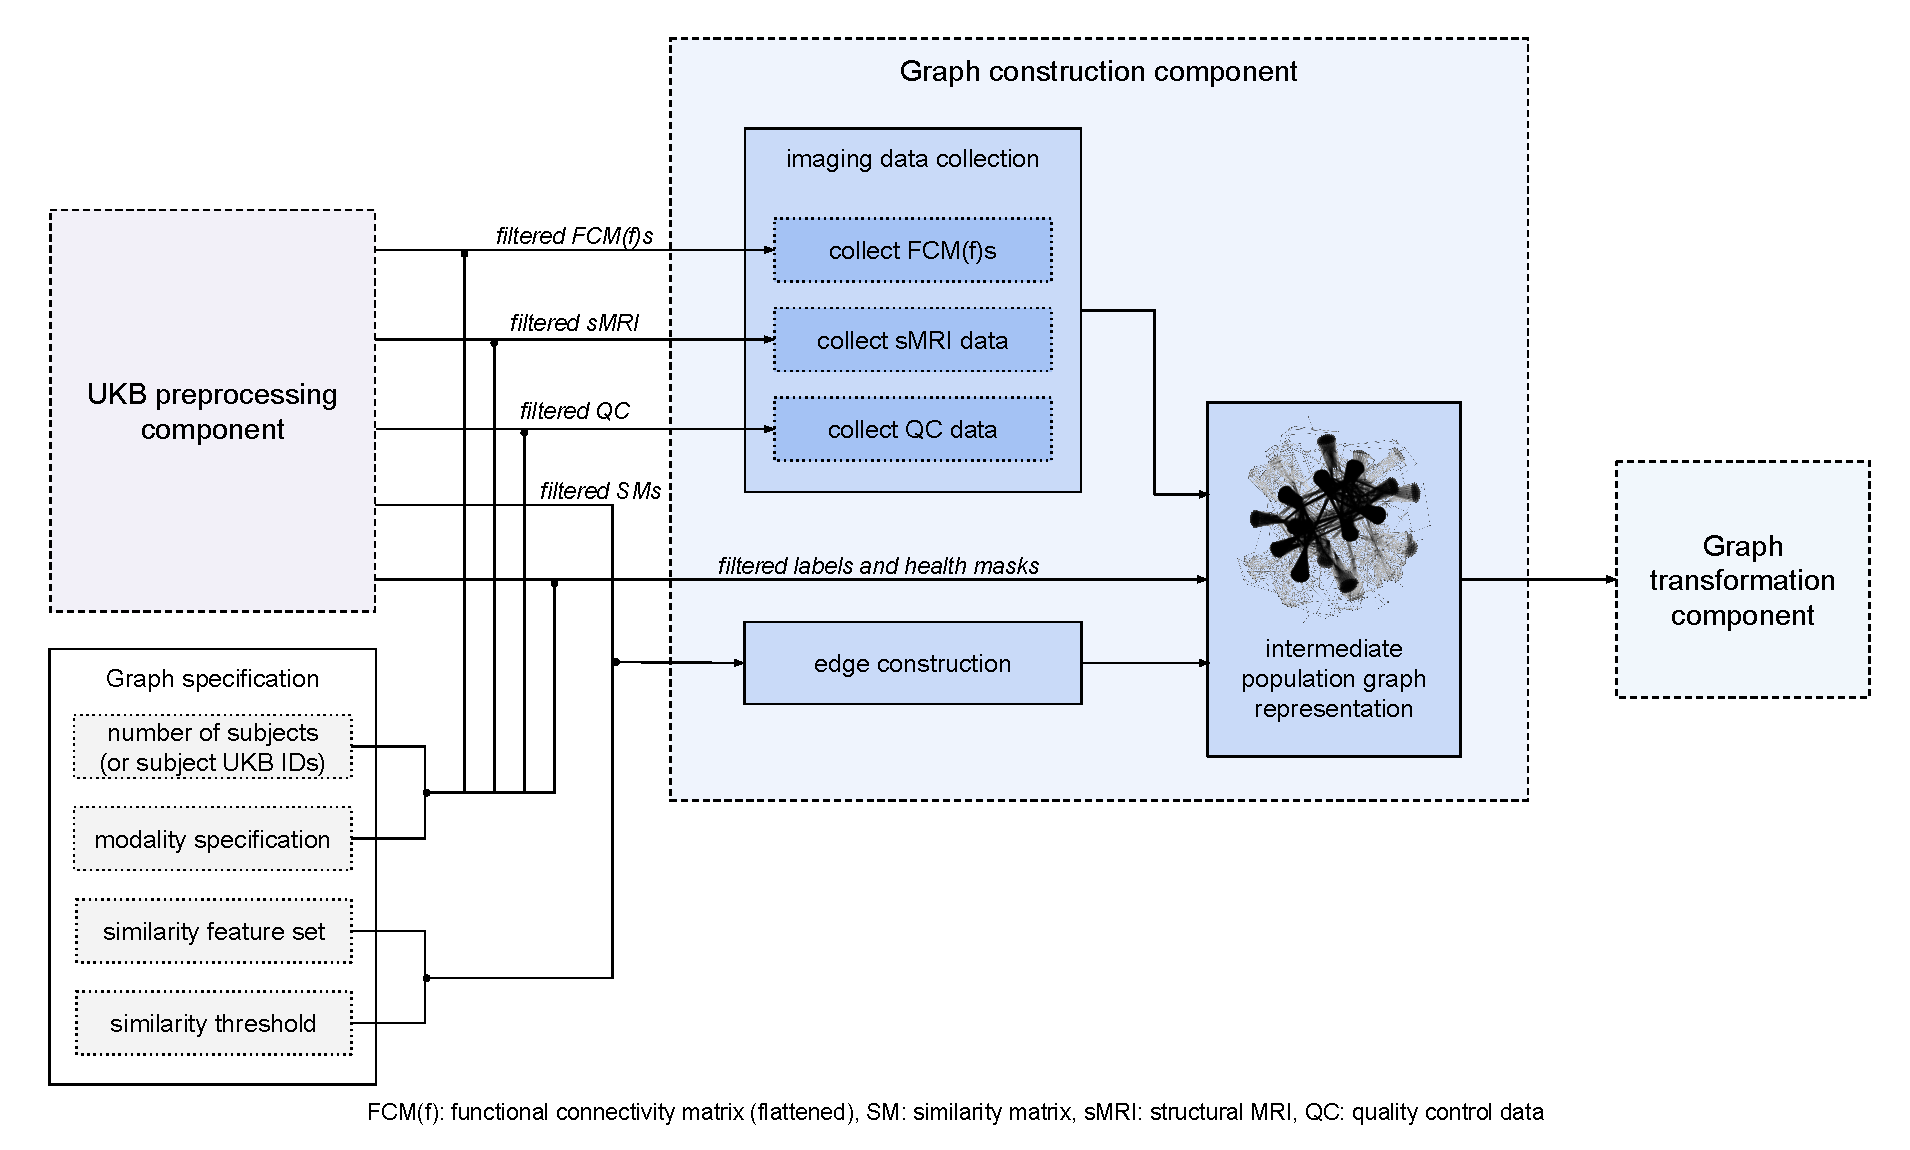
\includegraphics[width=\textwidth]{graph_construction_component.pdf}
    \caption{Graph construction component.}\label{graph-construction-component}
\end{figure}

\subsection{Inputs}
The inputs to the graph construction component can be categorised into four types as shown in the white box at the bottom left of Figure~\ref{graph-construction-component}:
\begin{enumerate}
    \item \textit{Modality specification} describes which of the neuroimaging modalities should be used as node features. This could be any combination of functional, structural and quality control data.
    \item \textit{Subject specification} takes in the number of (randomly selected) subjects that should be used to create the graph, or a list UKB identifiers for a graph containing a particular set of subjects. If no such parameter is provided, then all available data (filtered by the subject index described in the previous component) is used for population graph construction.
    \item \textit{Similarity specification}. 
    In its default implementation, the similarity score is computed as the average over a set of similarity features $\{M_1, \dots, M_n\}$ (see Equation~\eqref{eq:similarity}), in which case it is sufficient to specify the similarity feature set to be used. An \textit{extension} to this is to accept an arbitrary linear combination of various similarity features, allowing for much richer similarity metrics. 
    \item \textit{Similarity threshold}. A number $\mu \in [0,1]$ defining the threshold for the similarity metric above which an edge will be added to the graph (see Equation~\eqref{eq:similarity-threshold}).
\end{enumerate}


\subsection{Imaging data collection}

Based on the subject and modality specification, the relevant imaging data is collected from the raw UKB files (first filtered by subject index) and stored in the intermediate representation as a \textit{dataframe} (\texttt{pandas.DataFrame} object) indexed by UKB subject identifier. This is represented by the connections between UKB preprocessing component, graph specification and the blue imaging data collection box in Figure~\ref{graph-construction-component}. 

If a particular modality is unused, the dataframe stored is empty.

\subsection{Edge construction}

The edge construction component uses the subject specification, similarity specification, and the filtered similarity matrix data to find the similarity scores for each pair of subjects. Whenever the similarity score between two subjects exceeds the threshold, an undirected edge is added to the population graph. The edges are stored in a \textit{tensor} (\texttt{torch.tensor}), which is a PyTorch datatype for multi-dimensional matrices\footnote{\url{https://pytorch.org/docs/stable/tensors.html}}.

\subsection{Brain health mask computation}

Due to the nature of the brain age problem, the population graph can only be trained on subjects with healthy brains, although it may contain both healthy and non-healthy subjects. The \textit{brain health mask} is computed to determine which subjects can be included in training and which cannot. In particular, non-healthy subjects are not included in loss function computation, so that the \textit{direction} of parameter update depends on healthy subjects only while the entire graph is updated. As a result, the predicted labels are available for both healthy and non-healthy subjects, but because of the brain health mask the prediction corresponds to the brain age rather than chronological age, as discussed in Section~\ref{brain-age-estimation}.

In this project, the \textit{brain health} is approximated by the absence of diagnoses related to mental health or nervous system disorders, defined by the \texttt{ICD10}-similarity metric (see Table~\ref{table:phenotype-features}).

\subsection{Population graph representation}
\label{section:population-graph-representation}

The population graph is stored in an extended \texttt{torch\_geometric.Data} object\footnote{\url{https://pytorch-geometric.readthedocs.io/en/latest/modules/data.html}}, with its most important fields listed in Table~\ref{table:population-graph}. The intermediate population graph representation has all of its entries defined except for the feature vector \texttt{x} and the training, validation and test masks.

\setlength{\LTpost}{0pt}
\renewcommand{\arraystretch}{1.25}
% \begin{table}[]
%     \caption{The population graph data structure (excludes helper or utility fields).}\label{table:population-graph}
%     \centering
%     \begin{tabular}{lp{0.2\textwidth}p{0.5\textwidth}}
%         \hline
\begin{center}
\begin{longtable}[]{lp{0.175\textwidth}p{0.475\textwidth}}
    \caption{The population graph data structure (excludes helper or utility fields).}\label{table:population-graph}\\
    \hline \textbf{Field name} & \textbf{Type} & \textbf{Description} \\
    \hline
    \endfirsthead
    \multicolumn{3}{c}%
    {\tablename\ \thetable\ -- \textit{Continued from previous page}} \\
    \hline
    \textbf{Field name} & \textbf{Type} & \textbf{Description} \\
    \hline
    \endhead
    \hline \multicolumn{3}{r}{\textit{Continued on next page}} \\
    \endfoot
    \hline
    \endlastfoot
    % \texttt{num\_nodes} & long & Number of nodes (subjects) in the population graph. \\
    \texttt{subject\_index} & string array & UKB identifiers of the subjects. Stored in the same subject order as training masks, feature and label tensors; corresponds to the edge start and end values. \\
    \texttt{edge\_index} & $2\times 2|E|$ \hfill\newline long tensor & \texttt{edge\_index}$[0][i]=s_v$ and \hfill \newline \texttt{edge\_index}$[1][i]=s_w$ indicate a directed \hfill \newline edge $s_v \leadsto s_w$. To represent the undirected edge $(s_v, s_w) \in E$, the second directed edge $s_w \leadsto s_v$ is added. \\
    \texttt{functional\_data} & dataframe & Row-indexed by subject with columns containing the flattened functional connectivity matrix entries. Empty if no functional data is used in the population graph. \\
    \texttt{structural\_data} & dictionary of \hfill \newline dataframes & Dictionary is indexed by the structural data modality, in this case cortical thickness, surface area, and grey matter volume. The corresponding dataframes are row-indexed by subject with columns containing the features of the relevant structural data modality. The dataframes are empty if no structural data is used. \\
    \texttt{quality\_control\_data} & dataframe & Row-indexed by subject with the columns containing Euler indices for the left and right hemispheres of the brain. Empty if no quality control data is used. \\
    \texttt{x} & $N \times F$ \hfill\newline float tensor & \textit{Unused at the intermediate stage.} Contains the full normalised feature vector (of $F$ features) for every graph node (subject). \\
    \texttt{y} & $N \times 1$ \hfill \newline float tensor & Contains the labels of training data, in this case chronological age. \\
    \texttt{brain\_health\_mask} & boolean array & \texttt{True} indicates that the subject has a healthy brain and can be used for training, and \texttt{False} otherwise. \\
    \texttt{train\_mask} & boolean tensor & \textit{Unused at the intermediate stage.} \texttt{True} if the subject belongs to the training set, and \texttt{False} otherwise. \\
    \texttt{validation\_mask} & boolean tensor & \textit{Unused at the intermediate stage.} \texttt{True} if the subject belongs to the validation set, and \texttt{False} otherwise. \\
    \texttt{test\_mask} & boolean tensor & \textit{Unused at the intermediate stage.} \texttt{True} if the subject belongs to the test set, and \texttt{False} otherwise.
    % \end{tabular}
\end{longtable}
\end{center}

\section{Graph transformation component}

The graph transformation component is responsible for preparing the intermediate population graph representation for training by defining its normalised, concatenated feature vector as well as training, validation and test masks. The schematic diagram representing the population graph transformations in this component is shown in Figure~\ref{graph-transformation-component}.

\begin{figure}[h]
    \centering
    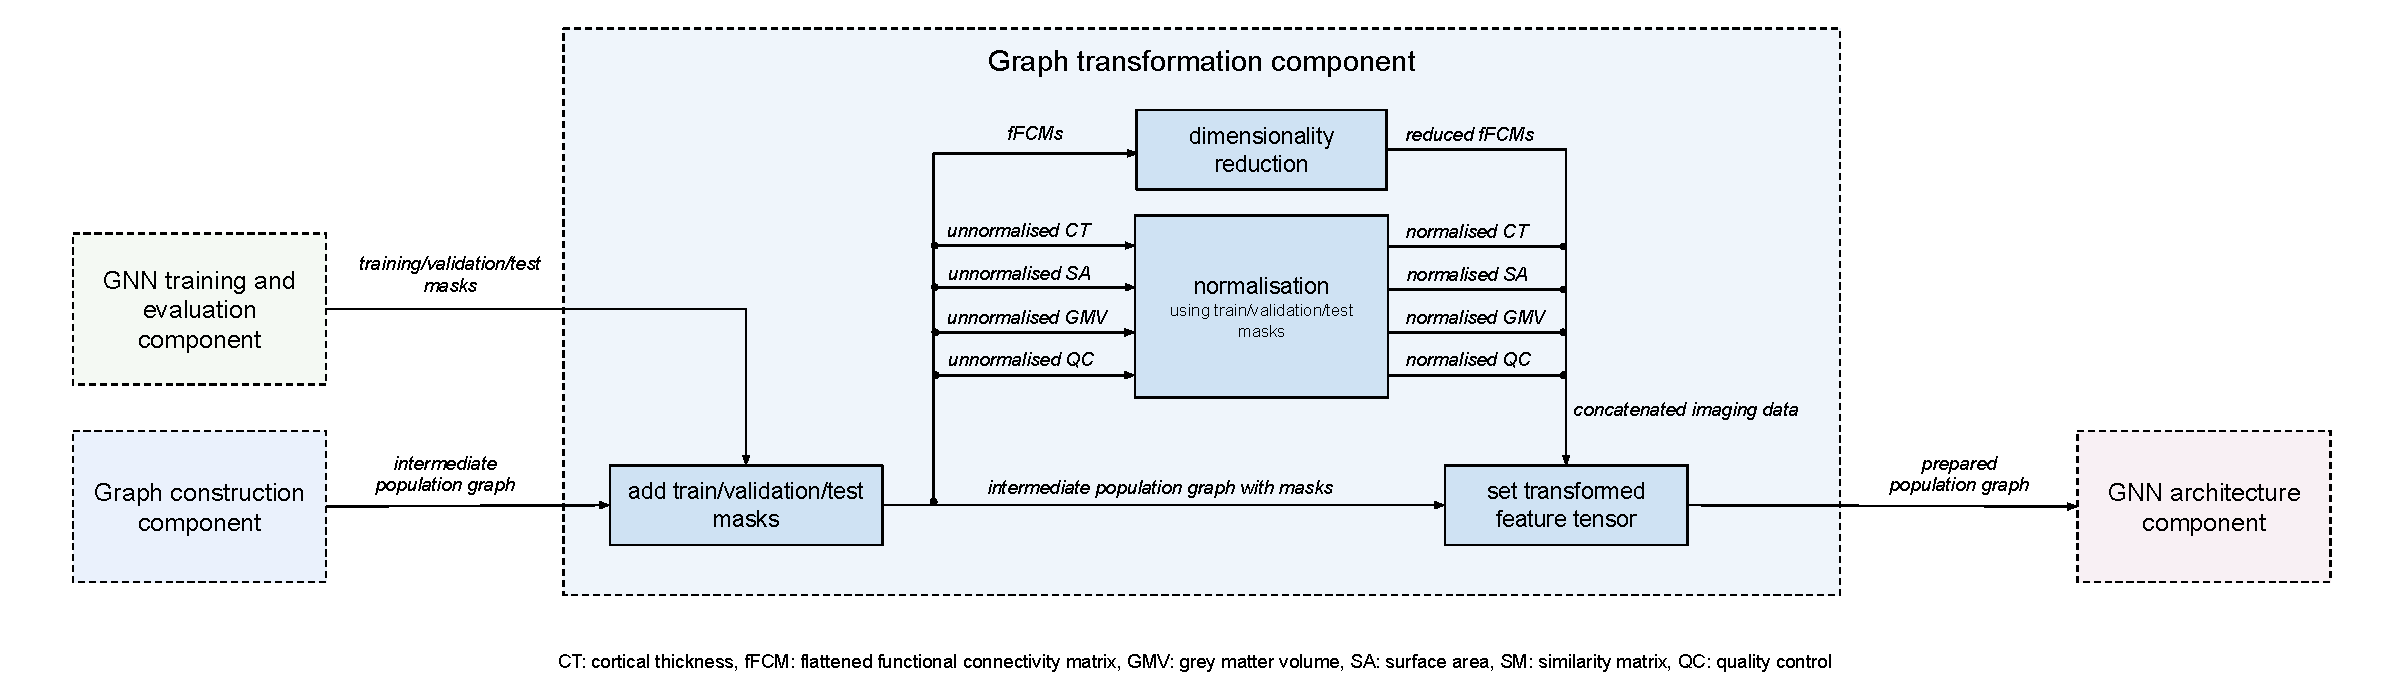
\includegraphics[width=\textwidth]{graph_transformation_component.pdf}
    \caption{Graph transformation component.}\label{graph-transformation-component}
\end{figure}

\subsection{Setting the training masks}
The first operation for preparing the population graph for training involves setting the \texttt{train\_mask}, \texttt{validation\_mask} and \texttt{test\_mask} fields of the intermediate population graph data structure (see Table~\ref{table:population-graph}). 

Following the brain age estimation method (Section~\ref{brain-age-estimation}), the masks are intersected with the \texttt{brain\_health\_mask}. Similarly to the reasoning behind the brain health masks, the three training masks are used to determine which nodes should be used to compute the loss function during various stages of training. For example, the model parameters are only updated based on the loss function for the subjects filtered with the \texttt{training\_mask}, and validation loss is computed only for the subjects filtered with the \texttt{validation\_mask}.

\subsection{Functional connectivity matrix dimensionality reduction}
The flattened functional connectivity matrix results in over 75,000 features per patient. Since the population graph cannot be split into parts and during training must be kept entirely in memory, along with all model parameters, this quickly runs into memory issues when the entire dataset is used. To mitigate this issue, some techniques may be applied to reduce the dimensionality of functional data. This project uses principal component analysis (PCA) as the dimensionality reduction technique of choice as it is one the simplest to implement. When the functional data is used to construct the population graph, PCA transformation is fitted to the training set as specified by the \texttt{training\_mask}, and the same transformation is applied to the remaining subjects. This dimensionality reduction technique is optional, and it is possible to define how many principal components should be kept after the transformation to control the amount of dimensionality reduction.

\subsection{Structural MRI and quality control data normalisation}
Next, the raw features stored under \texttt{structural\_data} and \texttt{quality\_control\_data} are normalised to be in the range between $-1$ and $1$ with mean 0. Similar to the previous section, standard scaler is fitted to the training set and applied to the validation and test sets. A separate transformation is applied to each structural data modality and the quality control modality.

\subsection{Setting the transformed feature tensor}
The transformed functional, structural and quality control modalities are concatenated together into a single tensor, which is assigned to \texttt{x} in the population graph data structure (Table~\ref{table:population-graph}). This makes it a prepared graph for training.

Since the original neuroimaging dataframes and brain health masks are kept in the data structure, the same population graph can be prepared for, say, a different training fold by simply going through the transformation component again but with a different training mask set, which will reset the values in the corresponding population graph fields.

\section{GNN architecture component}
% TODO not sure what exactly to write in this section. Past dissertations I've read seem to consider the hyperparameter tuning strategy, regularisation and in general description of hyperparameters that will be tuned. Another possiblity would be to explain in detail the implementation of the layers, but I'm not sure whether it's worth doing it because 1) it's a lot of words 2) it's in the library, not \textit{my} implementation 3) I already explain what the layers do in preparation. Maybe instead explain how the data is sent to wandb and how the training is performed.

% gcn_train(graph, device, n_conv_layers=0, layer_sizes=None, epochs=3500, lr=0.005, dropout_p=0, weight_decay=1e-5,
% log=True, early_stopping=True, patience=10, delta=0.005, cv=False, fold=0, run_name=None,
% min_epochs=1000):

\begin{center}
    \begin{longtable}[]{p{0.275\textwidth}p{0.175\textwidth}p{0.475\textwidth}}
        \caption{The parameters for the \texttt{BrainGNN} module.}\label{table:braingnn}\\
        \hline \textbf{Parameter} & \textbf{Type} & \textbf{Description} \\
        \hline
        \endfirsthead
        \multicolumn{3}{c}%
        {\tablename\ \thetable\ -- \textit{Continued from previous page}} \\
        \hline
        \textbf{Parameter} & \textbf{Type} & \textbf{Description} \\
        \hline
        \endhead
        \hline \multicolumn{3}{r}{\textit{Continued on next page}} \\
        \endfoot
        \hline
        \endlastfoot
        
        \texttt{conv\_type} & string & Indicates the type of graph convolutional layer to be used (graph convolution or graph attentional layer). \\
        \texttt{layer\_sizes} & integer array & Lists the number of units in every hidden layer. The length of the array corresponds to the total number of hidden layers. \\
        \texttt{n\_conv\_layers} & integer & Number of convolutional layers. Must be in range $[0, \text{\texttt{layer\_sizes}}]$. The sizes of those layers are determined by the first \texttt{n\_conv\_layers} values of the \texttt{layer\_sizes} and \texttt{n\_node\_features} parameters. \\
        \texttt{num\_node\_features} & integer & Indicates the number of input features. \\ 
        \texttt{dropout\_p} & float & The probability of ignoring the node in a hidden layer. Used as a regularisation technique to reduce overfitting.
    \end{longtable}
    \end{center}

The graph neural network component simply contains the implementations for the graph neural network (GNN) architectures used in this project: the graph convolutional network (GCN, Section~\ref{training-gcn}) and the graph attention network (GAT, Section~\ref{training-gat}). The networks are implemented as two PyTorch modules called \texttt{BrainGCN} and \texttt{BrainGAT}, which extend the more generic \texttt{BrainGNN} module. Table~\ref{table:braingnn} presents the parameters used to define a \texttt{BrainGNN} instance. \texttt{BrainGCN} and \texttt{BrainGAT}  have identical structure except that the \texttt{conv\_type} parameter is instantiated to \texttt{GCN} and \texttt{GAT} respectively, and the convolutional layers are set to either \texttt{torch\_geometric.nn.GCNConv} or \texttt{torch\_geometric.nn.GATConv} layers, both implemented in PyTorch Geometric library.

TODO perhaps simplify this? I don't know which parts to cut out of this for it to be clearer – what's unnecessary? I could also write pseudocode but not sure where it falls in the clarity vs professional spectrum. I could also delete the initialisation as I still plan to make a diagram for it – just not sure how to visualise how the \textit{array of parameters} is used.

\bigskip
\begin{code}
\caption{Simplified code snippet for \texttt{BrainGNN} instantiation and training.}
\label{listing:braingnn}
\medskip
\inputminted[frame=bottomline, linenos, breaklines=true, numberblanklines=false, style=colorful]{python}{code/brain_gnn_snippet.py}
\end{code}

Listing~\ref{listing:braingnn} shows how the order in which the layers are combined in the \texttt{BrainGNN} architecture, given the parameters in Table~\ref{table:braingnn}. I chose the hyperbolic tangent $\tanh(\cdot)$)as the non-linearity (activation function) between each layer because the inputs and values in neurons may be negative, in which case the other popular activation functions such as $\mathrm{ReLU}(\cdot)$ would have an undesirable asymmetric response. The \textit{dropout} layers have been added between the every fully connected layer as a regularisation technique: with probability \texttt{dropout\_p}, a unit in the layer is ignored at training time (its weight is zeroed) with the hope that the neural network will not rely on any particular node when predicting age, learning more robust features.


\section{GNN training and evaluation component}

\begin{figure}[]
    \centering
    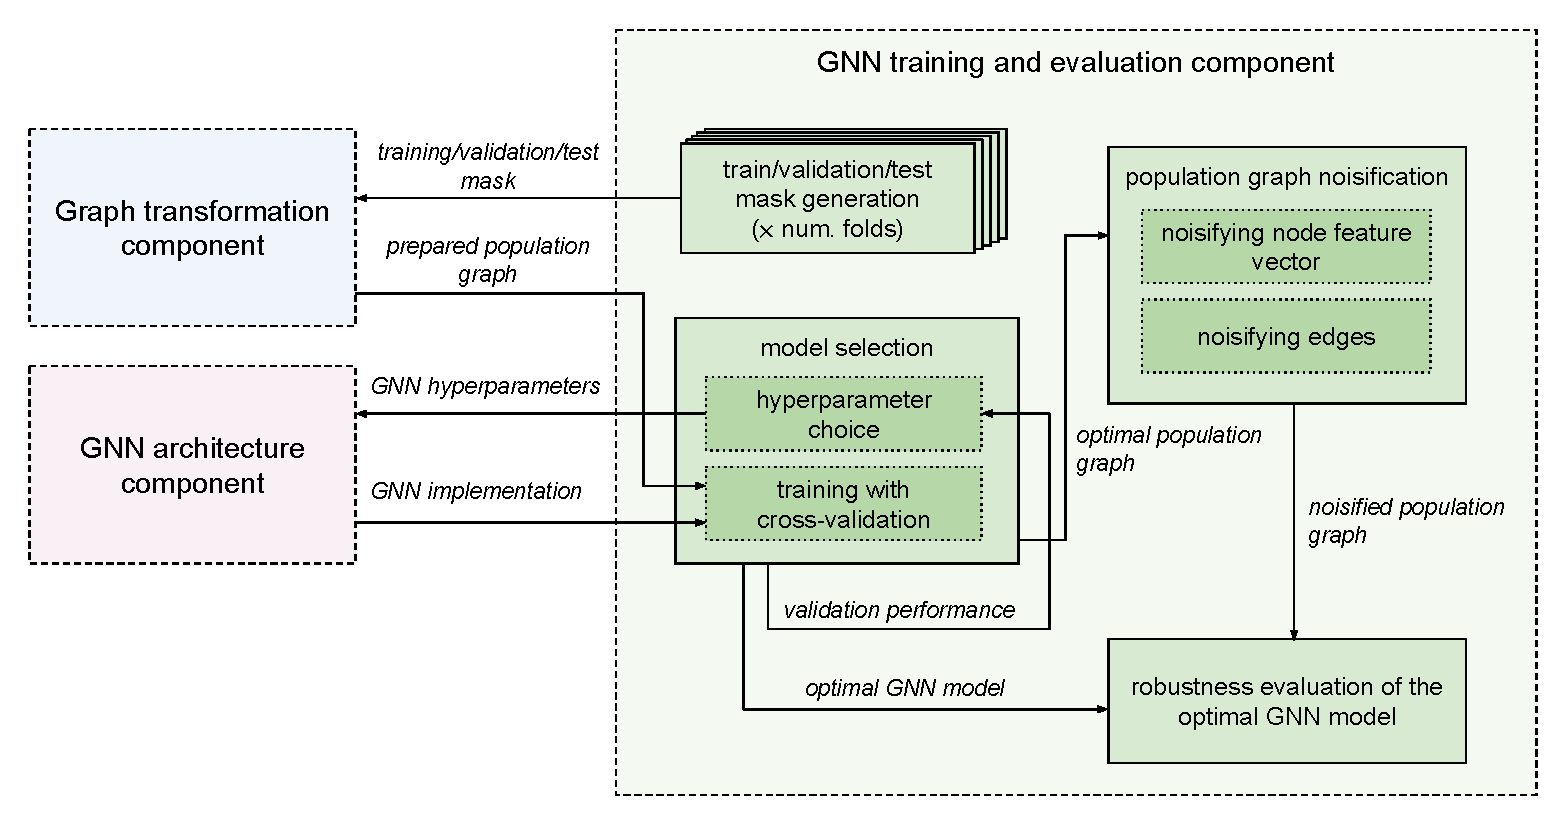
\includegraphics[width=\textwidth]{gnn_training_eval_component.pdf}
    \caption{Graph neural network training and evaluation component.}\label{gnn-training-eval-component}
\end{figure}

The main function of the GNN training and evaluation component is to select the best combination of population graph and GNN hyperparameters for each of the GCN and GAT architectures and report the results of the best model. A further \textit{extension} to this is the \textit{robustness evaluation} component, where robustness in this project is defined as the rate of the predictive power drop as noise is added to the population graph nodes or edges. The schematic overview of the GNN training and evaluation component is shown in Figure~\ref{gnn-training-eval-component}.


\subsection{Model selection}
% Hyperparameter tuning, weights and biases

With a high range of population graph modality (functional, structural, quality control data), similarity metric (Table~\ref{table:phenotype-features}), similarity threshold, as well as the GNN construction (Table~\ref{table:braingnn}) and training parameter (such as learning rate and number of epochs) choices, the search space for the best performing model is vast and it may be out of scope of this project to find the best fitting model.

TODO  I don't know whether the department likes something written in the first person. But I think is the first time you use this, so maybe doublecheck or think about it
The search space might be even bigger considering that I do not use all the possible non-imaging features in Table~\ref{table:phenotype-features} and there might be more confounders. There could be more similarity functions and the relative weights for each similarity feature – the subject's sex is probably more important than how many years they had of full-time education, for example. The UK Biobank has 768 non-imaging features per patient – it's out of scope to select the best ones and their relative weights and thresholds, especially having no neuroscience expertise etc\dots


Nonetheless I selected the set of features that I felt were the most important and carried out the hyperparameter tuning over the selected ranges of features.

\subsubsection{Mitigating memory constraints}
\label{section:memory}
The biggest constraint in training the population graphs was GPU memory (which accounting for intensive GPU usage in the laboratory was up to 5-8 gigabyte models, and often even 1-3 gigabyte models). This especially affects the population graph training since in this case, to train on the full dataset, the entire graph of more than 17,000 subjects must be in memory at once due to subject similarity connections, and unlike in most models that have individual independent examples, the population graph cannot be trivially split into smaller batches. At the same time, GCN and GAT are known to be memory-intensive models.
TODO reference
I wanted to use the entire dataset (
TODO why? – because the (quality of) data is often more important than the model, reference?),
which meant that I had to constrain my model and population graph structure selection instead. I constrained it as follows:

TODO "I decided" is def not a good wording here... try to make it just a normal, direct consequence from what you've read in the literature
\begin{enumerate}
    \item Having referred to the literature on brain age estimation, I decided that high-dimensional functional imaging data modality is less promising than structural imaging data modality, while adding a lot of extra features per patient (over 78,000). Functional imaging data is never used alone (especially because it's already very much an estimate of how the brain works and includes a lot of oversimplified assumptions to how the brain is connected, and if used, it is generally to only complement structural data). Dimensionality reduction is possible, but from experience from the practical work of my Data Science Unit of Assessment, PCA, for example, cutting out half of the low-variance principle components can even worsen the predictive power and training time of the model instead of improving it. While the support for those techniques is implemented – which indeed was the goal of this project to support it if it is needed – it was not used in training.
    \item The model size was fixed to a fairly shallow network with a small number of units (
        TODO give the actual architecture). 
        The learning rates were decreased and epochs increased to compensate for the smaller number of training parameters.
    \item I fixed the set of possible population graph types and the similarity thresholds (
    TODO see full list in Appendix ?). 
    From running some initial models I found that feasible similarity thresholds are all above 0.6, and even 0.7 or 0.8 often cause problems. 
\end{enumerate}


Hyperparameter search was restricted to only use the default similarity metrics for a more consistent training and because it is not clear how each metric should be weighted. The intent behind supporting this is the capability for a neuroscientist or another professional with domain knowledge to design their own good similarity metric – which has been implemented as an \textit{extension} to my original success criteria. Otherwise the weighting would be very arbitrary and increase the search space even more. As someone without much neuroscience domain knowledge I went for the simplest way of combining the metrics for this training procedure.

TODO in general lessons learnt and things for the future is that the memory issues and uninformed similarity metric and GNN architecture decisions severely restricted my hyperparameter search space, and very likely missed out on promising models with good test set performance. When I have time I would love to explore more hyperparameter options, consulting Dr Bethlehem and other experts on what other non-imaging features to include, how to combine them, how to adjust the architecture, and test new models on new data, for example on the recent UKB update which I did not have access to before, or some entirely new dataset. Alternatively, I could try training higher range of model hyperparameters on subsets of the UKB dataset, e.g. on 2,000-brain graphs which would decrease the parameters but allow for better exploration of the similarity matrix and GNN architecture possibilities.


\subsubsection{Hyperparameter tuning}
TODO is this implementation or evaluation? I feel like I could move it to evaluation so that I can show the results over each fold and how I selected them, not sure.

With the above GNN hyperparameter and population graph parameter restrictions due to memory constraints, I optimised the remaining hyperparameters using Bayesian optimisation strategy using the \textit{Sweeps} tool provided by the \textit{Weights~\& Biases}~\cite{wandb} (\texttt{wandb}) machine learning tracking and optimisation framework. 

TODO this is simplified – not sure how much do I want to explain the Gaussian processes etc.
Having integrated the training with the \texttt{wandb}, the framework would automatically suggest and test the best hyperparameter combinations it believes are the most likely to optimise the performance metric of choice, which in my case was to minimise the average cross-validation mean squared error (MSE). 

I ran the sweeps for both GCN and GAT models for at least 100 runs (most of them still unsuccessful due to the memory constraints) until the models started to converge to similar performance that could not be improved with new hyperparameters, and selected the best one for each architecture based on the lowest MSE.

TODO The hyperparameters tuned, their distributions and value ranges tuned can be found in Appendix ?.

TODO where to include this??? The models are trained using early stopping with patience of 100 and delta 0.005. This means that the training stops if the validation set MSE does not decrease by at least 0.005 in 100 consecutive epochs, at which point the model is reverted back to the state that gave the best validation set score). Otherwise, the models are trained for at least 1000 epochs and for a maximum of 7500 epochs.

\subsubsection{Cross-validation}
The subjects are first split into the 90\% training and 10\% hold-out test set, stratifying by subject age and sex. The test set will be used to evaluate a single selected model. 

The remaining data was used for model selection (hyperparameter tuning). The models were trained with five-fold cross-validation, so that the training data split into five folds with 90\% true training and 10\% validation subjects. Therefore for a given set of hyperparameters five models are trained, and the model's overall performance is estimated using the average mean squared error across the folds as well as the variation in performance. 

As the hyperparameter tuning converges, the most promising model is selected to be tested on the hold-out test set. The metrics usually used to evaluate the models performing a regression task are Pearson's correlation $r$ and coefficient of determination $r^2$.

\subsection{Robustness measurement}


The standard performance metrics $r$ and $r^2$ tracked and logged with training.

Describe the additional graph transformation stages which add noise to node features/edges.


\section{Repository overview}
% The repository overview should be around one page in length and should describe the high-level structure of the source code found in your source code Repository; ... could be implemented as a table with folders/file names and the functionality implemented in those files



\chapter{Evaluation}
\label{chapter:evaluation}
% This is where Assessors will be looking for signs of success and for evidence of thorough and systematic evaluation as discussed in Section 8.3. Sample output, tables of timings and photographs of workstation screens, oscilloscope traces or circuit boards may be included. A graph that does not indicate confidence intervals will generally leave a professional scientist with a negative impression.
% As with code, voluminous examples of sample output are usually best left to appendices or omitted altogether.
% There are some obvious questions which this chapter will address. How many of the original goals were achieved? Were they proved to have been achieved? Did the program, hardware, or theory really work?
% Assessors are well aware that large programs will very likely include some residual bugs. It should always be possible to demonstrate that a program works in simple cases and it is instructive to demonstrate how close it is to working in a really ambitious case.

% ~2,000 words

\section{Model ranking and selection}
\label{section:model-ranking}
Following the hyperparameter tuning process described in Section~\ref{section:training-procedure}, the models were selected according to the following procedure (applied separately to the GCN and GAT model families):
\begin{enumerate}
    \item First, the models were ranked by ascending average MSE loss. The model with the lowest average MSE was chosen as the reference model.
    \item All models whose 1 standard deviation interval from their MSE did not overlap with the 1 standard deviation interval of the reference model MSE were excluded from ranking.
\end{enumerate}

The cross-validation performance of the best-scoring models selected by the above procedure is shown in Figure~\ref{figure:gat-gcn-rank}. The hyperparameters for each of the short-listed models are listed in Tables~\ref{table:shortlisted-gcn} and~\ref{table:shortlisted-gat} (Appendix~\ref{appendix:hyperparameters}).

% \begin{figure}[]
%     \centering
%     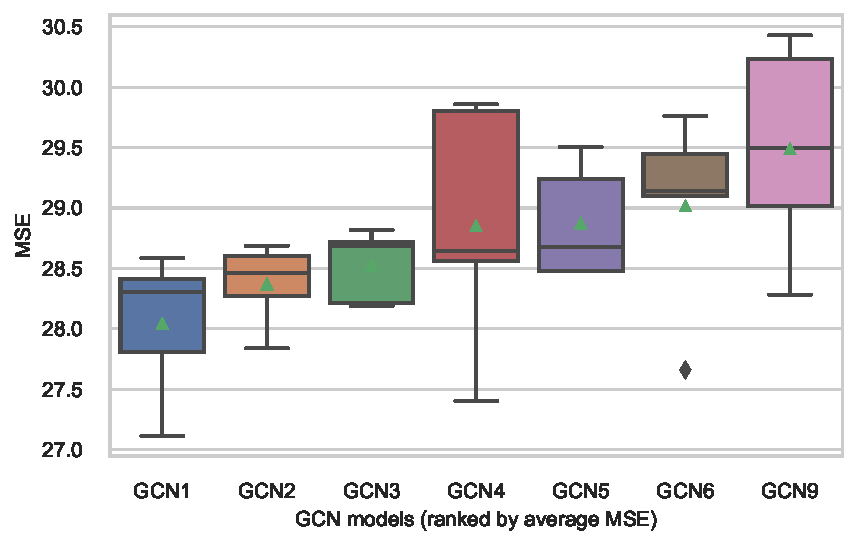
\includegraphics[width=\textwidth]{gcn_model_selection.pdf}
%     \caption{Highest scoring population graph and GCN model parameter combinations.}\label{figure:gcn-rank}
% \end{figure}

% \begin{figure}[]
%     \centering
%     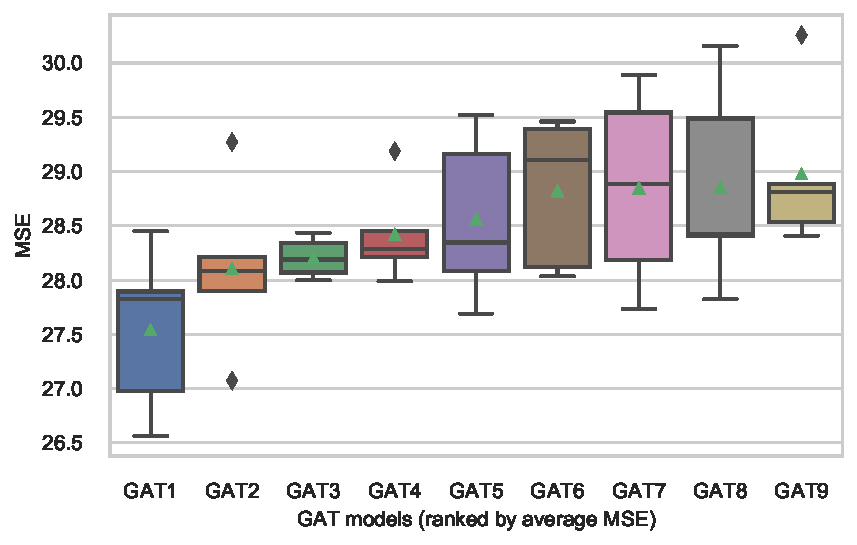
\includegraphics[width=\textwidth]{gat_model_selection.pdf}
%     \caption{Highest scoring population graph and GAT model parameter combinations.}\label{figure:gat-rank}
% \end{figure}

\begin{figure}[h]
    \centering
    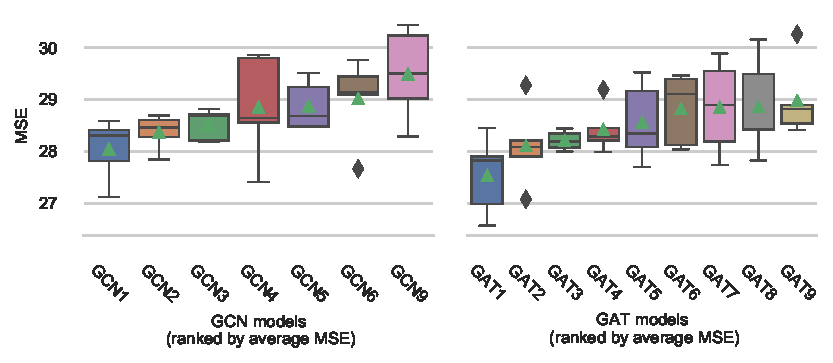
\includegraphics[width=\textwidth]{model_selection.pdf}
    \caption{Highest scoring population graph and GNN model parameter combinations.}\label{figure:gat-gcn-rank}
\end{figure}

Although both best-ranked (reference) models (GCN1 and GAT1) have relatively high variance, they still seem to be the most promising and therefore have been selected for further evaluation. Their population graph specification and GNN architecture hyperparameters are listed in Table~\ref{table:best-hyperparameters}.

\begin{table}[]
    \caption{Best performing population graph and GNN model parameter combinations during the model selection process.}\label{table:best-hyperparameters}
    \centering
    \small
    \begin{tabular}{p{0.3\textwidth}p{0.3\textwidth}p{0.3\textwidth}}
        \hline
    \textbf{Hyperparameter} & \textbf{GCN1} & \textbf{GAT1} \\  \hline
        Similarity feature set & \texttt{FI}, \texttt{FTE}, \texttt{ICD10}, \texttt{MEM}, \texttt{SEX} & \texttt{FI}, \texttt{ICD10}, \texttt{MEM}, \texttt{SEX} \\
        Similarity threshold & 0.9 & 0.8 \\ \hline
        Layer sizes & [1024, 512, 512, 256, 256, 1] & [2048, 1024, 512, 256, 128, 1] \\
        \# convolutional layers & 5 & 2 \\
        Dropout & $3.22 \times 10^{-1}$ & $3.14 \times 10^{-3}$ \\
        Learning rate & $6.98 \times 10^{-3}$ & $1.34 \times 10^{-2}$ \\
        Weight decay & $1.31 \times 10^{-2}$ & $6.05 \times 10^{-4}$ \\ \hline
\end{tabular}
\end{table}

\section{Evaluation metrics}
\label{section:evaluation-metrics}
The main performance metrics used for most regression problems, including brain age estimation task, are \textit{Pearson's correlation} and \textit{coefficient of determination}.

\subsubsection{Pearson's correlation}
For sets of true labels $\mathbf{y}  = [y_1 \dots y_N]$ with mean $\bar{y}$ and predicted labels $\mathbf{\hat{y}} = [\hat{y}_1 \dots \hat{y}_N]$, \textit{Pearson's correlation} is computed as

\begin{equation}
    r(\mathbf{y}, \mathbf{\hat{y}}) = \frac{\mathrm{cov}(\mathbf{y}, \mathbf{\hat{y}})}{\sigma_{\mathbf{y}} \sigma_{\mathbf{\hat{y}}}},
\end{equation}

where $\mathrm{cov}(\cdot, \cdot)$ denotes covariance and $\sigma$ stands for standard deviation. 

\subsubsection{Coefficient of determination}
The \textit{coefficient of determination} indicates how much variance in the features $\mathbf{X}$ could be explained by the model. It is computed as 
\begin{equation}
    r^2 = 1 - \frac{\sum_{i} (y_i - \bar{y})^2}{\sum_{i} (y_i - \hat{y}_i)^2}.
\end{equation}

Higher values for both metrics (with maximum 1) indicate a higher level of agreement between the true and predicted labels and therefore higher predictive power.


\section{Test set performance of selected models}
Generally in literature, after using cross-validation for model selection, the model is retrained on the entire dataset before giving a point estimate on a hold-out test set~\cite{raschka2018model}. This is because training on more data, especially when the dataset is small, allows to learn more patterns and therefore give better predictions on the unseen data. However, in this project the validation set was also used for early stopping since neural networks are especially prone to overfitting~\cite{prechelt1998automatic}. Some investigation of the hyperparameter tuning has shown that applying the stopping criteria discussed in Section~\ref{section:training-procedure} on just the training set would have still led to convergence only after the model has already overfit on the unseen validation labels. On the other hand, it is unclear how the stopping criteria should be adjusted when the training set size increases. 

Considering that the UKB dataset is large and that retraining the model with more data but without early stopping might not pay off for the loss in generalisation, all cross-validation folds were kept for test set performance estimation. Table~\ref{table:test-performance} gives the hold-out test set estimates for the metrics discussed in Section~\ref{section:evaluation-metrics}.

\begin{table}[h]
    \caption{Test set performance of GCN and GAT models.}\label{table:test-performance}
    \centering
    \small
    \begin{tabular}{ccc}
        \hline
    \textbf{Model} & $r$ & $r^2$ \\  \hline
        GCN1 & $0.675 \pm 0.008$ & $0.445 \pm 0.010$ \\
        GAT1 & $0.670 \pm 0.005$ & $0.477 \pm 0.008$ \\ \hline
\end{tabular}
\end{table}


\section{Significance testing of model performance}
\subsection{Experimental setup}
A classical test for assessing whether the models have truly learnt the relationships between the input features and the response variable is called a \textit{permutation test}~\cite{ojala2010permutation}. The null hypothesis assumes that features and labels are independent (i.e. that there is no relationship between the neuroimaging and non-imaging data and brain age), and the distribution corresponding to this hypothesis is estimated by randomly permuting the labels in the dataset. The $p$-value for this test is computed as

\begin{equation}
    p = \frac{\sum_{i=1}^k \mathbf{1}\left[\mathcal{L}(\mathbf{\hat{y}}, \pi(\mathbf{y})) \leq \mathcal{L}(\mathbf{\hat{y}}, \mathbf{y})\right] + 1}{k+1}\label{eq:p-value}
\end{equation}

where $\mathcal{L}(\cdot, \cdot)$ error function used to train the model (in this project MSE), $\pi(\cdot)$ indicates a permutation function which uniformly returns a random permutation of the argument, and $k$ is the number of samples.

In this project, $k=1000$ samples will be taken for each model family and the results will be claimed significant if the $p$-value in Equation~\eqref{eq:p-value} falls below the significance level $\alpha=0.05$. 

\subsection{Results}
The null distributions of GCN and GAT model errors with permuted labels are shown in Figure~\ref{figure:permutation-test}, with the MSE for the original dataset indicated by the red line.

\begin{figure}[h]
    \centering
    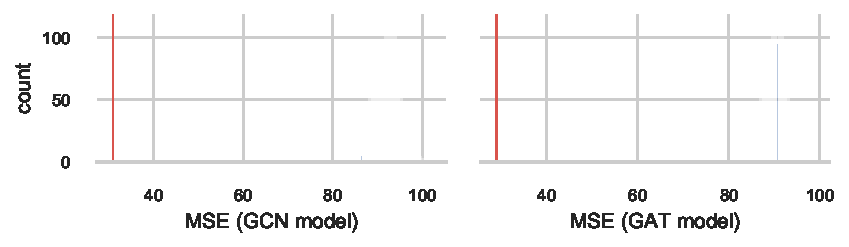
\includegraphics[width=\textwidth]{permutation_test.pdf}
    \caption{The null distribution of the label permutation test for GCN and GAT models. The red lines indicate MSE for the original dataset.}\label{figure:permutation-test}
\end{figure}

The $p$-values, representing how likely it is to get the MSE lower than the original dataset MSE purely by chance, were equal to $p=0.001$ for both GNN models. This is lower than the chosen significance level $\alpha=0.05$ so the null hypothesis is rejected and the performance of both models is statistically significant.


\section{GNN robustness to noisy population graph features}
\label{section:node-noise}
A desirable property for the real-world machine learning models is their robustness, defined as tolerance to the noise and inconsistency in data.
For population graphs trained on graph neural networks, this could be estimated by exploiting the neighbourhoods that are hopefully less noisy than a given node. Whether they are actually capable of doing so could be tested by adding noise to an increasing proportion of nodes. 

\subsection{Experimental setup}
For the feature noise robustness evaluation, an increasing proportion of population graph nodes is corrupted by randomly permuting their features. Then the model is retrained and tested on the hold-out test set, measuring the change in performance. To make sure that any effect on the evaluation metrics is due to added noise and not the changing dataset split, the model is trained on a single dataset split while the noise is added to different subjects. Moreover, to ensure that the effect on test set performance is due to the interaction with neighbourhoods and not due to the individual node features, only the nodes in the training set will be corrupted. For each of the GCN and GAT models, the experiment is repeated five times for each noise level (1\%, 5\%, 10\%, 20\%, 30\%, 50\%, 80\%, and 95\% of training nodes).

\subsection{Results}

The results of corrupting the node features on the predictive power of GNN models are shown in Figure~\ref{figure:node-noise}.

% \begin{figure}[h]
%     \centering
%     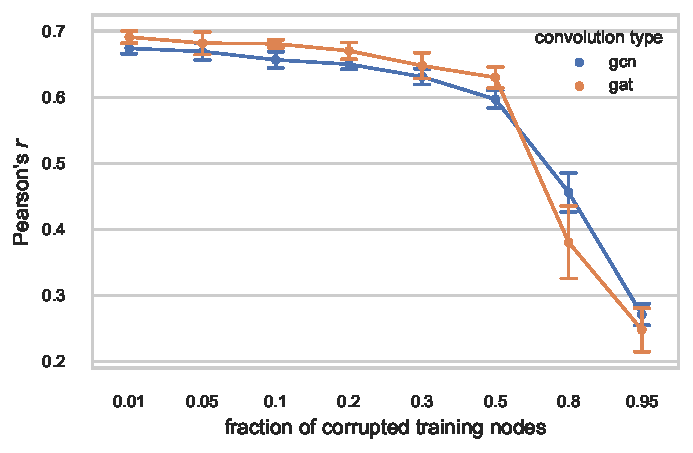
\includegraphics[]{node_noise_r.pdf}
% %     \caption{The effect of permuting node features on $r$ performance metric, with error bars representing standard deviation}\label{figure:node-noise-r}
% % \end{figure}

% % \begin{figure}[h]
% %     \centering
%     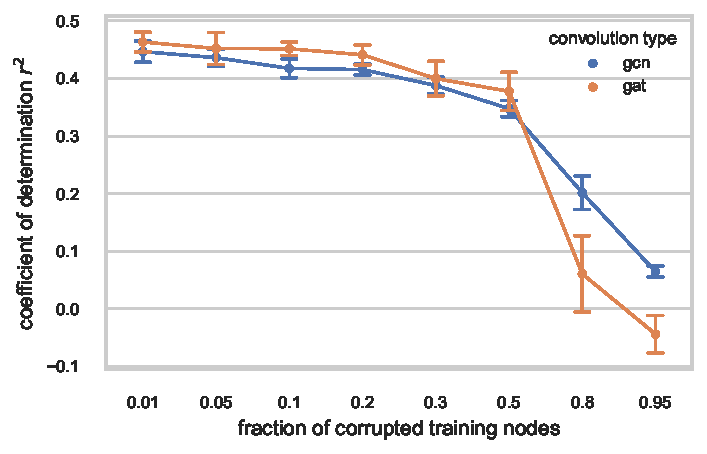
\includegraphics[]{node_noise_r2.pdf}
%     \caption{The effect of permuting node features on $r$ and $r^2$ performance metrics, with error bars representing standard deviation.}\label{figure:node-noise}
% \end{figure}

\begin{figure}[h]
    \centering
    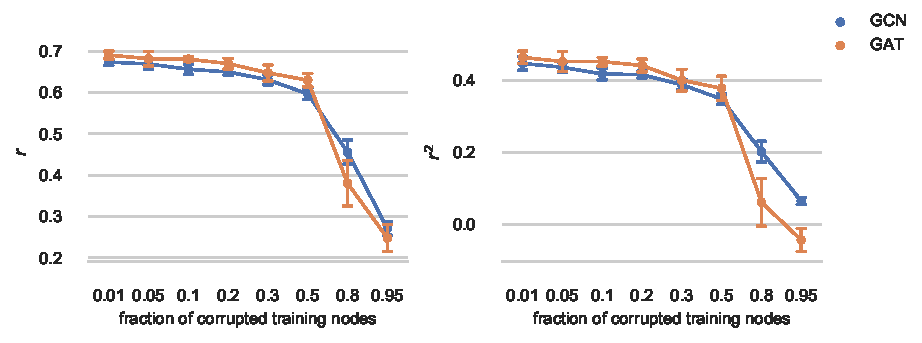
\includegraphics[]{node_noise.pdf}
    \caption{The effect of permuting node features on $r$ (left) and $r^2$ (right) performance metrics, with error bars representing standard deviation.}\label{figure:node-noise}
\end{figure}

As expected, for both GCN and GAT models the performance was decreasing relatively slowly as more training nodes got corrupted, and then dropped drastically when more than half of the training nodes had their features permuted. In case of the GAT model, the $r^2$ metric even fell below 0 (bottom of Figure~\ref{figure:node-noise}), which means that no variance could be explained and that the mean of the observed subject ages in the dataset is a better estimate of the brain age than the prediction of the GAT model. 

It is also possible to compare the relative GCN and GAT performance. While in this experiment the GAT model has higher (but similar) average scores at low noise levels, its performance drops faster, creating a wider gap between the scores, which could suggest that the GAT model is less robust to increasing noise. 

% \subsection{Discussion}
% In practice, in a big and well-curated dataset such as the UK Biobank, the existence of exact protocols for equipment and measurement taking should prevent there being too many unacceptably noisy scans. Even in that case, the noise would take a milder form than the complete shuffling of features that make the node data meaningless. Having that considered, at low proportions of added noise, both models have been able to retain most of their predictive power, which could indicate their generalisability to new contexts.


\section{GNN dependence on population graph similarity metrics}
\subsection{Experimental setup}
The assumption behind the population graph model is that the edge structure helps to control for confounding effects while giving additional information which could be useful for brain age prediction. One experiment to test this is to remove an increasing proportion of edges from the population graph, with the proportions of removed edges being the same as in the previous section. The training procedure is then repeated five times at each edge loss level using a different random seed. The more edges are removed, the less neighbourhood structure the graph neural network models can exploit, having to rely on individual node features. 

\subsection{Results}
The effect of removing the edges on predictive power of the GNN models is shown in Figure~\ref{figure:edge-noise}. Compared to the results in Section~\ref{section:node-noise} where the predictive power drastically dropped with increased noise, the loss of information contained in edges and neighbourhoods of similar nodes did \texttt{not} affect the predictive power of the models. This could be inferred from the standard deviation intervals being quite wide for both evaluation metrics, overlapping across most, if not all, edge loss levels.

% \begin{figure}[]
%     \centering
%     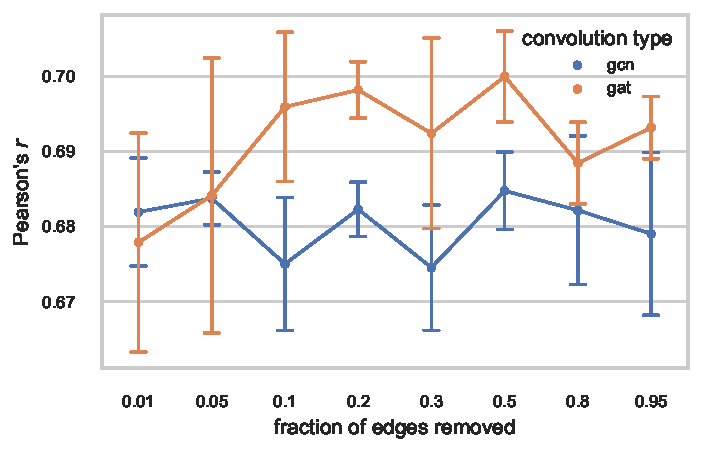
\includegraphics[]{edge_noise_r.pdf}
% %     \caption{The effect of removing edges on $r$ performance metric, with error bars representing standard deviation}\label{figure:edge-noise-r}
% % \end{figure}

% % \begin{figure}[h]
% %     \centering
%     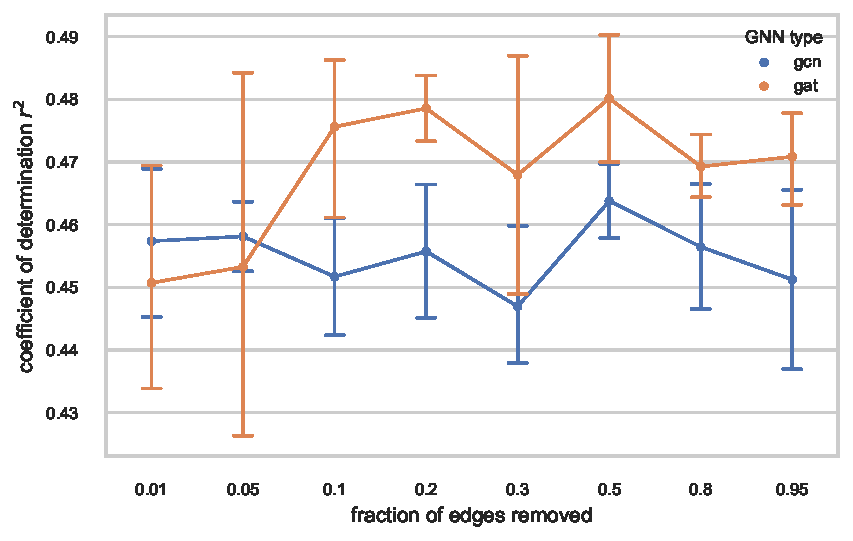
\includegraphics[]{edge_noise_r2.pdf}
%     \caption{The effect of removing edges on $r$ and $r^2$ performance metrics, with error bars representing standard deviation.}\label{figure:edge-noise}
% \end{figure}

\begin{figure}[h]
    \centering
    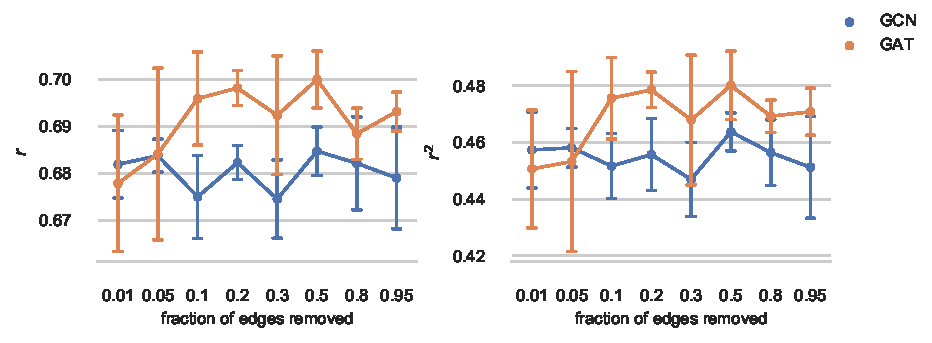
\includegraphics[]{edge_noise.pdf}
    \caption{he effect of removing edges on $r$ (left) and $r^2$ (right) performance metrics, with error bars representing standard deviation.}\label{figure:edge-noise}
\end{figure}


\section{Discussion}
 The edge removal experiment shows that for brain age estimation problem, the models relied more on the features of individual nodes rather than similarity metrics and in turn the neighbourhoods of other population graph nodes. This might mean that the similarity metrics were not informative enough to allow for effective sharing of feature and/or label information, or that the (brain) age depends more on the feature interactions within a single brain rather than particular signals that generalise to other individuals. Moreover, the node noisification experiment shows that the neighbours could be even \textit{harmful} as, due to experimental setup, the changes in performance in Figure~\ref{figure:node-noise} are only due to the changes in neighbouring nodes but not in the test nodes themselves.

If this is true, more powerful models that do not use the graph structure might be more appropriate for the brain age estimation task. This is consistent with considerably better brain age estimation performance of other non-GNN models found in literature (such as $r=0.93$ in Kaufmann et al.~\cite{kaufmann2019} using an XGBoost model, and $r=0.94, r^2=0.88$ in Cole et al.~\cite{cole2018brain} using a Gaussian process regression model), and even ``consistently poor'' performance of GNN models when applied to a similar task (to the point that in Pervaiz et al.~\cite{pervaiz2020optimising} the GNN results were dropped altogether from further discussion).


% \section{Comparison against existing benchmarks}

% Compare to the Kaufmann et al.'s \textit{xgboost} approach \cite{kaufmann2019} ($r \sim 0.93$); and the other package that was cited in the same paper.
% Possibly compare to other non-graph (relatively baseline) (neural network) architectures, e.g. ElasticNet, MLP,...



\chapter{Conclusion}

% This chapter is likely to be very short and it may well refer back to the Introduction. It might properly explain how you would have planned the project if starting again with the benefit of hindsight.

%  ~500 words

\section{Success criteria}
The project has achieved and exceeded all of its success criteria and requirements (Section~\ref{section:requirements-analysis} and Project Proposal, Appendix~\ref{chapter:project-proposal}), representing the UKB dataset as a population graph, implementing the two GNN frameworks, and evaluating their results. It has made a lot of progress on its proposed extensions, measuring the significance and robustness of the GNN models and increasing the flexibility of the preprocessing pipeline to more preprocessing options.

\section{The main contribution}
The main success and contribution of this project was its step towards a preprocessing pipeline that could leverage several brain imaging and non-imaging modalities at once in a unified and consistent manner. This is important in neuroimaging research regardless of the downstream task or analysis method, as there is a widespread community effort to combat the neuroimaging reproducibility crisis~\cite{gorgolewski2016practical} caused by, among other factors, the lack of transparency in preprocessing methods and software errors due to bad software engineering practices~\cite{poldrack2017scanning}.
% \footnote{\url{http://reproducibility.stanford.edu/about-us/}}
% Even for the same dataset, the preprocessing workflow alone could significantly affect the results~\cite{salehi2020there}, and the workflows (particularly for functional data) may vary significantly between different research teams~\cite{botvinik2019variability}. 

While the efforts to improve reproducibility of neuroimaging research are currently targeted at consistent processing of functional and structural MRI with libraries such as \textit{fMRIPrep}~\cite{esteban2019fmriprep} and \textit{Pypes}~\cite{savio2017pypes}, this project, to the best of my knowledge, is one of the first to additionally incorporate non-imaging data modalities. While it was designed to prepare the data specifically for population graphs, due to its modular structure it has sufficient flexibility to be easily extended to more preprocessing options and modalities, and adapted to work independently of the downstream analysis method.

\section{The main lessons}
This interdisciplinary project has been exploring two things – the brain age estimation problem, and graph neural networks as a way of solving it. Both of the machine learning and neuroimaging fields are currently at the height of their ongoing research, with some of the literature this project relied on being only a few months old~\cite{kaufmann2019, niu2019improved, pervaiz2020optimising}. The continuous collaboration with experts from both disciplines was an enriching experience; more importantly, however, this guidance was crucial to ensure that my work is not only a technically challenging, but also a clinically relevant contribution to the neuroscience community.

At the same time, this project taught me first-hand an important lesson in approaching predictive analysis problems in real-world settings. While the goal of this project was to learn more about the advanced, cutting-edge methods in computational neuroscience, and to get hands-on experience with the tools for implementing them, the development of models \textit{in practice} should consider the simplest approaches first and only then apply the more sophisticated techniques. This was demonstrated by conceptually simpler methods in literature outperforming the more complex architectures proposed in this project. I am particularly proud of implementing what I called the robustness measurement framework – it insightfully showed that the graph neural network models did not rely on the similarity metrics as it was expected, naturally suggesting a direction for future work.

\section{Directions for future work}
To make this work more accessible to the wider neuroimaging community, the most important future direction would be to create an interface to the preprocessing pipeline that is agnostic to the downstream analysis task and make it publicly available online.

While it was not practical to do this extension for the UKB dataset that uses its own organisation and preprocessing steps, the preprocessing pipeline could be adapted to work with raw magnetic resonance images, which would make it applicable to many more neuroimaging datasets and parcellations (that would now be a part of the preprocessing framework). This could be especially useful in a more general clinical setting where image acquisition is not standardised and the neuroimaging preprocessing expertise might not be available. 
% The preprocessing framework is also a project that could benefit from good software engineering and computer science skills in order to design a general pipeline that is efficient, flexible and simple to apply to different contexts.

Some parts of the preprocessing component (e.g. fMRI preprocessing) could be extended to use other existing libraries for reproducible research, with this pipeline offered as an extension. In case there are no existing libraries, the proposed pipeline could offer additional methods in a consistent and easy-to-use manner. Support for additional modalities – such as genetic data that has already proved to be useful for neuroimaging tasks~\cite{cole2018brain,parisot2018disease} – could also be implemented.


% TODO: you should mention in your future work that you've used a linear data reduction technique. Given how noisy and non-linear the fMRI is, future work should explore better ways to get a good representation of fmri timeseries, which maybe would help in this prediction task, but out of scope of dissertation
% Apr 23, 2020 1:31 AM
% Tiago Manuel: besides you are backed up by niu's paper saying that fmri might not be useful. but still the reasoning point of linear/non linear interactions maintains

% rb643: Again more for future implementation: I've been playing around with running PCA on the raw time-series as well as Diffusion Embedding on the connectivity matrices and they provide strikingly similar results. Thus is might be computationally efficient to use raw time-series PCA in the future. Generally only the first half dozen PC's are interesting anyway

% Mention Niu et al. 2019 raising the issue that there is systematic bias in brain age gap prediction but not many studies use this knowledge to correct for it. 

% * this pipeline allows to try out more different state-of-the-art GNN architectures and population graphs quickly and efficiently


% * opens up possibilities to incorporating new modalities at scale with growing datasets in the future

% 3) neuroscience findings
% this could be transfer the modular system for the different datasets (HCP)

%TC:ignore
%%%%%%%%%%%%%%%%%%%%%%%%%%%%%%%%%%%%%%%%%%%%%%%%%%%%%%%%%%%%%%%%%%%%%
\addcontentsline{toc}{chapter}{Bibliography}
\printbibliography

%%%%%%%%%%%%%%%%%%%%%%%%%%%%%%%%%%%%%%%%%%%%%%%%%%%%%%%%%%%%%%%%%%%%%

\appendix
% Assessors like to see some sample code or example circuit diagrams, and appendices are the sensible places to include such items. Accordingly, software and hardware projects should incorporate appropriate appendices. Note that the 12,000 word limit does not include material in the appendices, but only in extremely unusual circumstances may appendices exceed 10–15 pages – if you feel that such unusual circumstances might apply to you you should ask your Director of Studies and Supervisor to apply to the Chairman of Examiners. It is quite in order to have no appendices. Appendices should appear between the bibliography and the project proposal.


\chapter{Hyperparameter search}
\label{appendix:hyperparameters}

This Appendix contains the hyperparameter search configuration and the hyperparameters for the best performing models as selected in Evaluation procedure (Chapter~\ref{chapter:evaluation}, Section~\ref{section:model-ranking}).

\section{Hyperparameter tuning configuration}

\bigskip
\begin{code}
\caption{Hyperparameter search configuration for the GCN and GAT model families.}
\label{listing:sweep-config}
\medskip
\inputminted[frame=lines, linenos, breaklines=true, numberblanklines=false, style=colorful]{yaml}{code/sweep_config.yaml}
\end{code}

\section{Hyperparameters of shortlisted models}
Tables~\ref{table:shortlisted-gcn} and~\ref{table:shortlisted-gat} use encodings given in Tables~\ref{table:sf-encoding} and~\ref{table:ls-encoding} for similarity feature sets and layer sizes respectively.

\begin{table}[h]
    \caption{Similarity feature set encoding.}\label{table:sf-encoding}
    \centering
    \small
    \begin{tabular}{cccccc}
        \hline
    \textbf{Encoding} & \texttt{FI} &  \texttt{FTE}& \texttt{ICD10}& \texttt{MEM}& \texttt{SEX}\\  \hline
        SF1 & Yes & Yes & Yes & Yes & Yes \\
        SF2 & Yes & No & Yes & Yes & Yes \\
        SF3 & No & Yes & Yes & Yes & Yes \\
        SF4 & Yes & Yes & No & Yes & Yes \\ \hline
\end{tabular}
\end{table}

\begin{table}[h]
    \caption{Layer size encoding.}\label{table:ls-encoding}
    \centering
    \small
    \begin{tabular}{cccccc}
        \hline
    \textbf{Encoding} & \textbf{Layer sizes} \\  \hline
        LS1 & [1024, 512, 512, 256, 256, 1] \\ 
        LS2 & [1024, 512, 512, 512, 256, 256, 1] \\
        LS3 & [1024, 512, 256, 128, 128, 1] \\
        LS4 & [2048, 1024, 512, 256, 128, 1] \\
        LS5 & [512, 512, 512, 256, 128, 1] \\ \hline
\end{tabular}
\end{table}

\begin{sidewaystable}[h!]
    % \begin{table}[]
    \caption{Shortlisted population graph and GCN model parameter combinations during the model selection process.}\label{table:shortlisted-gcn}
    \centering
    \centering
    \small
    \begin{tabular}{lccccccc}
        \hline
    \textbf{Hyperparameter} & \textbf{GCN1} & \textbf{GCN2} & \textbf{GCN3} & \textbf{GCN4} & \textbf{GCN5} & \textbf{GCN6} & \textbf{GCN9} \\  \hline
        Similarity feature set &  SF1 & SF3 & SF3 & SF2 & SF2 & SF2 & SF2 \\
        Similarity threshold & 0.9 & 0.8 & 0.8 & 0.8 & 0.8 & 0.8 & 0.8\\ \hline
        Layer sizes & LS1 &  LS2 & LS3 & LS5 & LS3 & LS3 & LS4 \\ 
        \# convolutional layers & 5 & 3& 1& 2& 5& 3& 4\\ 
        Dropout &  0.321941 & 0.042080& 0.048596& 0.237940& 0.375442& 0.386998& 0.426491\\ 
        Learning rate & 0.006984& 0.006187& 0.005095& 0.004731& 0.015796& 0.010273& 0.003504\\ 
        Weight decay & 0.013118& 0.002084& 0.016171& 0.002517& 0.003114& 0.005341& 0.018943\\ \hline
\end{tabular}
 
\bigskip\bigskip

    \caption{Shortlisted population graph and GAT model parameter combinations during the model selection process.}\label{table:shortlisted-gat}
    \centering
    \small
    \begin{tabular}{lccccccccc}
        \hline
    \textbf{Hyperparameter} & \textbf{GAT1} & \textbf{GAT2} & \textbf{GAT3} & \textbf{GAT4} & \textbf{GAT5} & \textbf{GAT6} & \textbf{GAT7} & \textbf{GAT8} & \textbf{GAT9} \\  \hline
    Similarity feature set & SF2 & SF1 & SF2& SF1 & SF1& SF1& SF1& SF2& SF2\\
    Similarity threshold & 0.8 & 0.9& 0.8& 0.9& 0.9& 0.9& 0.9& 0.8& 0.8\\ \hline
    Layer sizes& LS4& LS3& LS3& LS5& LS3& LS3& LS3& LS5& LS5\\
    \# convolutional layers & 2& 2& 3& 2& 3& 2& 3& 3& 3\\
    Dropout & 0.003142& 0.306806& 0.104624& 0.327091& 0.407471& 0.323481& 0.291117& 0.455777& 0.381829\\
    Learning rate& 0.013365& 0.001679& 0.003412& 0.002482& 0.003246& 0.001462& 0.006769& 0.006813& 0.003820\\
    Weight decay& 0.000605& 0.002071& 0.036676& 0.001549& 0.006715& 0.002475& 0.000844& 0.001483& 0.003226\\ \hline
\end{tabular}
    \end{sidewaystable}

\begin{refsection}
% \documentclass[12pt,a4paper,twoside, hidelinks]{article}
% \usepackage{bookmark}
% \usepackage{amsmath}
% \usepackage{parskip}
% \usepackage{enumitem}
% \usepackage{hyperref}
% \urlstyle{same}
% \usepackage{xcolor}
% \usepackage[multiple]{footmisc}
% \usepackage[margin=25mm]{geometry}
% % \usepackage[backend=biber, maxnames=4]{biblatex}
% % \addbibresource{stankeviciute-proposal.bib}

% \begin{document}
\chapter{Project proposal}
\label{chapter:project-proposal}

\begin{center}
\Large
Computer Science Tripos -- Part II -- Project Proposal\\[4mm]
\LARGE
Graph neural networks for age prediction from neuroimaging data \\[4mm]

\large
2419E

% \today % October 2019
\end{center}

\vspace{5mm}
\textbf{Project Originator:} Tiago Azevedo

\textbf{Project Supervisors:} Tiago Azevedo, Alexander Campbell, Prof Pietro Liò

\textbf{Project Overseers:} Prof Jon~Crowcroft, Dr Thomas~Sauerwald

% Main document

\section*{Introduction}
% The problem to be addressed.

% [Tiago] Why NNs and not something else? You probably want one sentence of motivation saying they have been very successful in other fields, and then one sentence that as a consequence they might help physicians.
% \textit{...Neural networks provide the opportunity to capture the similarities between patients and trends which might help physicians to understand the mechanisms of the disease and in turn find more effective treatments...}

A graph neural network (GNN) is a type of a neural network that operates on graph inputs and is used for tasks like node classification, link prediction and clustering (geometric deep learning). GNNs have recently become popular and proved successful in a broad range of real-world applications, such as text and image classification, knowledge graphs, and interaction modelling in physical and biological systems. \cite{zhou2018gnn}

One domain where graphs offer a natural representation is social networks and \textit{populations}, with nodes representing individuals (their features and labels), and edges corresponding to associations between individuals according to some heuristic or a formally defined similarity metric. The reason why such graph representation is considered to be useful in the geometric deep learning context is that the network can make use of both the individual features (node feature vectors) and the overall trends in the population through pairwise similarities (graph edges), \cite{parisot2017spectral} inferring the label of an individual node both from the node itself and from its neighbourhood.
% The graph structure is also helpful when incorporating multiple modalities of data, which is often the case for medical records containing, for example, imaging and non-imaging data. 

\section*{Project description}
This project was inspired by Parisot et al.'s \cite{parisot2017spectral, parisot2018disease} state-of-the-art application of a type of a GNN called Graph Convolutional Network (GCN) to the population graphs of healthy controls and patients with neurological or neurodegenerative disorders. In these papers, the GCN (adapted from Kipf and Welling \cite{kipf2017semi}) was used in a semi-supervised manner for two classification tasks: 1) prediction of autism spectrum disorder (ASD) from the ABIDE dataset and 2) prediction of a progressive form of Mild Cognitive Impairment (MCI) that develops into Alzheimer's disease (AD) from the ADNI dataset.

Moreover, a recent paper by Kaufmann et al. \cite{kaufmann2019} has linked the incidence of common brain disorders, including ASD, MCI, and AD as well as others, to the deviation between chronological and biological brain ageing. These results suggest that being able to estimate the subject's age from the neuroimaging data may be important in understanding the mechanisms of those disorders and helping physicians to find more effective treatments.

The aim of this project will therefore be to adapt the population graph approach of Parisot et al. \cite{parisot2017spectral, parisot2018disease} to a regression task on the UK Biobank dataset, predicting the subject's age based on neuroimaging data, and comparing it to another successful geometric deep learning architecture such as the Graph Attention Network. \cite{velickovic2018graph} The performance of the networks will be evaluated on the standard metrics, e.g. the coefficient of determination~$r^2$.

\section*{Starting point}
% Describe existing state of the art, previous work in this area,
%   libraries and databases to be used. Describe the state of any
%   existing codebase that is to be built on.

The source code for the implementation of Kipf and Welling's \cite{kipf2017semi} GCNs and Parisot et al.'s \cite{parisot2017spectral, parisot2018disease} first classification task is publicly available online.\footnote{\url{https://github.com/tkipf/gcn}}\footnote{\url{https://github.com/parisots/population-gcn}}

I will be using PyTorch for this project because of its support for machine learning on structured graph data. In particular, PyTorch Geometric (PyG)\footnote{\url{https://github.com/rusty1s/pytorch_geometric}} – a geometric deep learning extension library – will make the implementation, iteration and extensions to the model more flexible in addition to performance improvements and simplified APIs.
% making the final library more accessible and extensible, contributing to the open-source community

I have experience with the basics of TensorFlow\footnote{Five-course Deep Learning specialisation by deeplearning.ai on Coursera}\footnote{Google's Machine Learning Crash Course and follow-up courses.} and no experience with PyTorch or graph neural networks. I have attended or will study (possibly in advance) the CST courses related to the subject of this project, such as IA Machine Learning and Real-World Data, IB Artificial Intelligence, II Data Science, II Bioinformatics, and II Machine Learning and Bayesian Inference.

\subsection*{Dataset}

I will be using the data from the UK Biobank, kindly preprocessed and provided by Dr~Richard Bethlehem of the Department of Psychiatry.

The UK Biobank is a large dataset containing comprehensive phenotypic, genetic, MRI and other data from the total of over 500,000 participants.\footnote{\url{https://www.ukbiobank.ac.uk/participants/}} In this project, I will be using the subset of this dataset with only those subjects who had the neuroimaging data collected and preprocessed (approximately 20,000 participants). This includes both structural (T1, T2 FLAIR) and functional (resting state fMRI) data, preprocessed with the standard UK Biobank pipelines\footnote{\url{https://biobank.ctsu.ox.ac.uk/crystal/crystal/docs/brain_mri.pdf}} and additionally denoised and parcellated (in several common parcellations) by Dr Bethlehem. 
% I am likely to be using the correlation matrices and raw parcellated time series for functional and features like coritical thickness for structural data.

\section*{Work to be done}
\label{section:work}

% [Tiago] bullet points should start with the same sentence structure

% Describe the technical work.
The following are lists of explicit deliverables to be implemented.

\textbf{Graph neural network framework}
\begin{enumerate}[label=G\arabic*.]
  \item The data is preprocessed into features and is ready for analysis. % [Tiago] "data cleaned and is ready for analysis" 
  \item Definition of the similarity metric to be used in connecting the graph. The graph is connected based on that similarity metric to be processed by graph neural networks.
  \item Implementation of Kipf's GCN \cite{kipf2017semi} for the age regression task.
  % [Tiago] GAT originally doesn't allow for weighted edges. You probably want to say GAT because of interesting results in previous literature. Thus, you can probably divide this point: (1) implementation of another graph NN layer, (2) Include weights (in theory you can even edit the message passing mechanism in GCN to multiply by the weights, just like you are suggesting for GAT) 
  \item Implementation of the Graph Attention Network for comparing its performance to the Graph Convolutional Network.
  % [Tiago] What exactly would you be testing points? Eg. what a unit test would consist of?
  % [Tiago] I just recalled that one thing we discussed could be how it handles missing data (eg. a certain percentage without some data), which could create an interesting view on robustness and semi-supervised learning. Maybe this could go to extension (or "personal" extension in case you have time and you can say you had one more extension than initially planned)
\end{enumerate}

\textbf{Evaluation framework}

\begin{enumerate}[label=E\arabic*.]
  \item  Comparison of the alternative graph neural network models using the coefficient of determination $r^2$.
\end{enumerate}

\section*{Success criteria}
% Describe what you expect to be able to demonstrate at the
% end of the project and how you are going to evaluate your achievement.
The project will be successful if the following items will have been implemented.
\begin{enumerate}[label=SC\arabic*.]
  \item Representation of the UK Biobank data as a population graph with nodes representing the individuals and edges representing associations between them based on pairwise similarity.
  \item The Graph Convolutional Network for age regression on the population graph.
  \item The Graph Attention Network for the same task.
  \item The evaluation framework for comparing the performance of the two graph neural networks.
\end{enumerate}

\section*{Evaluation of the project}
The performance of the graph neural networks will be measured across several metrics. The main metric to evaluate a regression task, in contrast the classification in Parisot et al. \cite{parisot2018disease}, is the coefficient of determination~$r^2$. 

\section*{Possible extensions}
% Potential further envisaged evaluation metrics or extensions.
\begin{enumerate}[label=PE\arabic*.]
  \item An additional metric that could be used to evaluate the performance of the networks is \textit{robustness} to missing or noisy data. Robustness, which could be defined as \textit{the rate at which the predictive power drops as more information is removed from the nodes}, would reveal how important is the neighbourhood (edge) information for accurate predictions compared to the node features only.
  \item Implement spectral filter computation with \textit{Cayley polynomials} instead of using Chebyshev polynomials. Cayley polynomials have been introduced in a paper by Levie et al. \cite{levie2017cayleynets} and were mentioned in Parisot et al. \cite{parisot2018disease} as a possible improvement.
  \item The main implementation of the graph neural network relies on manually handcrafted features from preprocessed brain imaging data. Time permitting, an extension could be to create a package that can be used after any standard neuroimaging preprocessing pipeline (e.g. with results in BIDS\footnote{\url{https://bids.neuroimaging.io}} format) to extract these features, and possibly improve upon as well as create new ones. This would make execution of the model more efficient, robust and generalisable.
  \item Implement weighted edges in the Graph Convolutional Network and Graph Attention Network, as the main implementations will have binary edges.
  % \item Implement a \textit{custom similarity metric}. The metrics used in the work by Parisot et al. \cite{parisot2018disease} were defined arbitrarily by the authors based on very few features. Learning a different similarity metric based on more combinations of features could possibly result in a better performance of the classifier.

\end{enumerate}


\section*{Timetable and milestones}
\label{section:timetable}

% A work plan of perhaps ten or so two-week work-packages,
% as well as milestones to be achieved along the way. Provide a
% target date for each milestone.

% [Tiago] you can specify which parts of the work you intend to implement in each 2-week time frame. This will help you having a better idea of how you are keeping up/behind.

%  (01/10/2019 – 16/10/2019)
\textbf{Michaelmas weeks 0–1}
\begin{itemize}
  \item Work on project proposal.
\end{itemize}

\textbf{Milestones.} Submit Phase 1 report by 14/10/2019. Submit draft proposal by 18/10/2019.

% (17/10/2019 – 06/11/2019)
\textbf{Michaelmas weeks 2–4}
\begin{itemize}
  \item Get access to the UK Biobank data and get familiar with its features.
  \item Define a possible graph similarity metric.
\end{itemize}

\textbf{Milestones.} Submit final project proposal by 25/10/2019.

% (07/11/2019 – 20/11/2019)
\textbf{Michaelmas weeks 5–6}
\begin{itemize}
  \item Write code for connecting the nodes based on a similarity metric.
  \item Connect the nodes (with their features) into a graph.
  \item Start working on the implementation of the Graph Convolutional Network (e.g. define loss and random label removal for semi-supervised training, start implementing the layers).
\end{itemize}

% (21/11/2019 – 04/12/2019)
\textbf{Michaelmas weeks 7–8} 
\begin{itemize}
  \item Work on the implementation of layers for the Graph Convolutional Network. Compute the general performance metrics.
  \item Start working on Graph Attention Network implementation for the same task.
\end{itemize}

\textbf{Michaelmas vacation}
\begin{itemize}
  \item Continue working on and finish the neural network implementations, compute performance metrics.
  \item Work on graph neural network evaluation: implement the robustness measurement framework.
  \item Measure the robustness of the neural networks.
  \item Start writing the dissertation and the project progress report.
\end{itemize}

\textbf{Milestones.} Complete the implementation of the main part of the project.

% (16/01/2020 – 29/01/2020)
\textbf{Lent weeks 0–2}
\begin{itemize}
  \item Finish the progress report, prepare for the presentation.
  \item Implement Cayley polynomials.
  \item Start working on the data preprocessing pipeline.
\end{itemize}
 
\textbf{Milestones.} Submit progress report by 31/01/2020.

% (30/01/2020 – 19/02/2020)
\textbf{Lent weeks 3–5}
\begin{itemize}
  \item Continue implementing the data preprocessing pipeline.
  \item Start working on the implementation of weighted edges.
\end{itemize}


% (20/02/2020 – 11/03/2020)
\textbf{Lent weeks 6–8}
\begin{itemize}
  \item Finish implementing the data preprocessing pipeline.
  \item Finish implementing the weighted edges.
  \item Continue working on the dissertation write-up.
\end{itemize}

\textbf{Easter vacation}
\begin{itemize}
  \item Complete the dissertation draft and send it for review.
  \item Edit the draft based on the feedback received.
\end{itemize}

\textbf{Milestones.} Send out the complete draft for review by 27/03/2020. Submit dissertation early by 20/04/2020.

% (24/04/2020 – 06/05/2020)
\textbf{Easter weeks 0–2}

 Time reserved for any unexpected issues.

 \section*{Resource declaration}

 For this project I will be using my personal MacBook Pro (2019, with 1.4 GHz Quad-Core Intel Core i5 processor and 8GB of RAM). Training the model will require the use of GPUs provided by the Computational Biology Group (as confirmed by Prof Pietro Liò). To prevent any loss of data, both the source code and the \LaTeX\ source will be stored on my machine, private GitHub repositories, and Google Drive, as well as regularly backed up on an external HDD.

% \medskip 
% \printbibliography

\printbibliography[title=References]
\end{refsection}
%TC:endignore

\end{document}
